\documentclass{_formatting}

%% ============================================================
%% Dodatkowe pakiety (ponad to, co ładuje klasa _formatting.cls).
%% Czcionki, język, marginesy, biblatex, hyperref, float, amsmath,
%% indentfirst, microtype i xcolor są ustawione w _formatting.cls —
%% nie ładujemy ich tu ponownie, aby nie nadpisywać formatowania.
%% ============================================================

\usepackage{graphicx}
\usepackage{needspace}
\usepackage{colortbl} % \rowcolor w tabelach (xcolor ładuje klasa)
%% amssymb pominięty — koliduje z unicode-math (klasa), który zawiera te symbole

%% cleveref musi być załadowany po hyperref (hyperref ładuje klasa)
%% jawna opcja języka — bez niej cleveref wywraca się przy polyglossia
\usepackage[english]{cleveref}

%% własne środowisko pływające „wykres” (pakiet float ładuje klasa)
\newfloat{wykres}{htbp}{low}[chapter]
\floatname{wykres}{Wykres}

%% źródło bibliografii (sam biblatex konfiguruje klasa)
\addbibresource{bibliography/references.bib}

\usepackage{glossaries}

\input{config/commands}
\title{System przetwarzania danych oparty na pojedynczym oraz współpracujących modelach LLM}
\author{
    Oliwier Komorowski
    \and
    Jakub Nowak
}
\date{\today}
\input{config/glossaery}

%% ustawienia formatowania dla dodatków (musi być przed \appendix)
%% ============================================================
%% Formatowanie nagłówka: „Dodatek A: Tytuł” 
%% Automatyczne dodanie do spisu treści
%% Zawartość pozostaw bez zmian
%% ============================================================

% zachowujemy domyślne ustawienia \chapter do późniejszego użycia
\makeatletter
\let\OrigChapter\chapter

%% stworzenie nowego polecenia \appchapter z numeracją literową
\NewDocumentCommand{\appchapter}{ m o }{
  \refstepcounter{chapter}
  \setcounter{section}{0}
  \gdef\currentchaptertitle{#1}
  \OrigChapter*{Dodatek~\thechapter: #1} % dopisanie "Dodatek" do tytułu
  \chaptermark{#1}
  \phantomsection
  \addcontentsline{toc}{chapter}{Dodatek~\thechapter: #1} % dodanie do spisu treści
  \IfNoValueF{#2}{\label{#2}}
}

%% po poleceniu \appendix
%% \chapter{...} korzysta z \appchapter,
%% \chapter*{...} działa jak dotąd (bez numeru w spisie treści).
\pretocmd{\appendix}{
  \let\OrigChapter\chapter
  \renewcommand{\chapter}{
    \@ifstar{\OrigChapter*}{\appchapter}
  }
}{}{}
\makeatother


\begin{document}

%% strony wstępne (kolejno: strona tytułowa, oświadczenie, streszczenie, wykaz symboli)

\includepdf[pages=-]{frontmatter/1_title.pdf}

\includepdf[pages=-]{frontmatter/2_statement.pdf}
%% ============================================================
%% STRESZCZENIE — OPIS FORMATKI
%% ============================================================
\chapter*{Streszczenie}
\phantomsection
\addcontentsline{toc}{chapter}{Streszczenie}

Projekt inżynierski dotyczy współpracy wielu dużych modeli językowych (LLM) w rozwiązywaniu złożonych problemów.

\section*{Słowa kluczowe:}
\noindent duży model językowy (LLM), współpraca wielu modeli, umysł rojowy, Ollama
\section*{Dziedzina nauki i techniki, zgodnie z wymogami OECD:}
\noindent Nauki o komputerach i informatyka

%% ============================================================
%% STRESZCZENIE PO ANGIELSKU — OPIS FORMATKI
%% ============================================================
\chapter*{Abstract}
\phantomsection
\addcontentsline{toc}{chapter}{Abstract}
This engineering project concerns the cooperation of multiple large language models (LLMs) in solving complex problems.

\section*{Keywords :}
\noindent large language model (LLM), multi-model collaboration, hive mind, Ollama
\section*{Field of science and technology in accordance with OECD requirements:}
\noindent Computer Science and Information Technology

%% ============================================================
%% Wykaz ważniejszych oznaczeń i skrótów
%% ============================================================

%% ------------------ Nagłówek + wpis do spisu treści -------------------
\chapter*{Wykaz ważniejszych oznaczeń i skrótów}
\phantomsection
\addcontentsline{toc}{chapter}{Wykaz ważniejszych oznaczeń i skrótów}

%% --------- Podstawowe wielkości i operatory ----------
%% Tabela 4 kolumny: symbol | jednostka | łącznik „--” | opis
%% Wyrównanie: l r c l (lewo, prawo, środek, lewo)
\section*{Podstawowe wielkości fizyczne oraz wyrażenia matematyczne}
\noindent
\begin{tabular}{l r c l}
     $j$  &$[\cdot]$  &--&jednostka urojona\\
	 $\nabla$  &$[\cdot]$  &--&operator nabla\\
	 $\vec{i}_{x},\vec{i}_{z},\vec{i}_{y} $ &$[\cdot]$  &--& wersory układu współrzędnych kartezjańskich    \\
	 $\vec{F}$ &$[\text{N}]$  &--& siła \\
	 $t $ &$[\text{s}]$  &--& czas \\
	 $m$  &$[\text{kg}]$  &--& masa \\
	 $R$  &$[\Omega]$  &--&rezystancja\\
	 $\mathbf{S}$  &$[\cdot]$  &--&macierz rozproszenia\\
\end{tabular}

%% -------------- Stałe i wartości znane ---------------
%% Tabela 4 kolumny: symbol/wartość | jednostka | łącznik | opis
\section*{Stałe fizyczne i matematyczne}
\noindent
	 \begin{tabular}{l r c l}
	$\pi \approx 3.14159 $&$[\cdot]  $ &--& liczba $\pi$\\ 
	$g \approx 9.80665 $&$[\frac{\text{m}}{\text{s}^2}]  $ &--& przyspieszenie ziemskie\\
\end{tabular}

%% ---------------- Terminologia użyta w pracy -----------------
%% Tabela 3 kolumny: komenda | łącznik „--” | objaśnienie
%% Użyte \verb|...| zabezpiecza zapis komend dosłownie.
%% \multirow rozszerza opis na kilka wierszy
\section*{Terminologia użyta w pracy projektowej}
\noindent
\begin{tabular}{l c l} 
\verb|\section{}| &--& tworzy tytuł rozdziału \\
\verb|\subsection{}|&--&  tworzy tytuł podrozdziału \\
\verb|\cite{}| &--& odwołanie do pozycji z bibliografii \\
\verb|\ref{}|&--&  odwołanie do rysunku, tabeli lub wzoru \\
\verb|\eqref{}| &--& odwołanie do równania (z nawiasem)  \\
\verb|\begin{figure}| & \multirow{3}{*}{--} & \multirow{3}{*}{wstawienie obiektu graficznego} \\
... & & \\ 
\verb|end{figure}| & & \\ 
\verb|\begin{table}| & \multirow{3}{*}{--} & \multirow{3}{*}{wstawienie tabeli} \\
... & & \\ 
\verb|end{table}| & & \\ 
\verb|\begin{equation}| & \multirow{3}{*}{--} & \multirow{3}{*}{wstawienie wzoru z numeracją} \\
... & & \\ 
\verb|end{equation}| & & \\ 
\verb|\textbf{}| &--& pogrubienie tekstu  \\
\verb|\emph{}| &--& wyróżnienie kursywą  \\
\verb|\footnote{}| &--& wstawienie przypisu dolnego \\
\verb|\includegraphics{}| &--& wstawienie obrazu \\
\verb|\label{}| &--& etykieta obiektu \\
\verb|\item| &--& element listy \\
\end{tabular}


%% -------------------- Spis treści ---------------------------
\renewcommand{\contentsname}{Spis treści}
\clearpage
\phantomsection
\addcontentsline{toc}{chapter}{Spis treści}
\label{page:Table_of_contents}
\tableofcontents

%% -------------------- Rozdziały główne ----------------------
% !TEX root = ../main.tex
\chapter{Wstęp i cel pracy}

Aktualnie duże model językowe (ang. LLM, Large Language Model) wykorzystywane są w różnych obszarach obszarach życia. Wysokie zainteresowanie sztuczną inteligencją sprzyja rozwojowi tej dziedziny. Skutkuje to pojawianiem się nowych możliwości wykorzystania technologii przetwarzania języka naturalnego oraz zrewolucjonizowaniem sposobu, w jakim systemy informatyczne przetwarzają i analizują dane nieustrukturyzowane. 

W miarę jak rosną oczekiwania wobec systemów opartych na LLM, pojedynczy model może okazać się niewystarczający. Typowymi ograniczeniami są koszt obliczeniowy pojedynczego zapytania czy podatność na błędy wynikające z braku weryfikacji własnych odpowiedzi. Naturalną odpowiedzią na te ograniczenia jest koncepcja architektur wielomodelowych, w których kilka instancji LLM współpracuje ze sobą.

\section{Motywacja}

Motywacją do realizacji projektu jest rosnące zainteresowanie sztuczną inteligencją, w szczególności dużymi modelami językowymi i ich możliwościami. Jednak główną motywacją jest sprawdzenie, czy dwa różne modele współpracując udzielą lepszych odpowiedzi niż pojedyńczy model.

\subsection{Dynamiczny rozwój dziedziny}

W ciągu ostatnich dekad można było zauważyć dynamiczny postęp w obszarze sztucznej inteligencji (SI, ang. Artificial Intelligence, AI). Rozwój tej dziedziny doprowadził do znacznego zwiększenia liczby prowadzonych na całym świecie badań, co znajduje odzwierciedlenie między innymi w rosnącej liczbie cytowań publikacji poświęconych tej tematyce. W ciągu ostatniej dekady sztuczna inteligencja (SI) rozwija się bardzo dynamicznie. Przełom przyniósł koniec 2022 roku, kiedy publicznie udostępniono ChatGPT. Prostota obsługi także dla osób bez wiedzy technicznej przyczyniła się do jego błyskawicznej popularności \cite{feuerriegel_generative_ai}. Szybki rozwój badań nad dużymi modelami językowymi (LLM) potwierdza przegląd ponad 5000 publikacji z lat 2017-2023 \cite{bibliometric_llm_review}. Generatywna SI (GenAI) znajduje zastosowanie m.in. w medycynie, edukacji, biznesie, inżynierii i tworzeniu oprogramowania oraz w generowaniu treści, w tym muzyki i wideo \cite{feuerriegel_generative_ai,bibliometric_llm_review}.

Jedną z dziedzin rozwijających się w ramach sztucznej inteligencji jest przetwarzanie języka naturalnego (ang. Natural Language Processing, NLP). Jej głównym zadaniem jest umożliwienie komputerom pracy z językiem używanym przez człowieka poprzez jego odpowiednie przekształcanie i interpretowanie. Pozwala to na automatyczną analizę, generowanie oraz przetwarzanie treści tekstowych. Istotnym elementem rozwoju NLP stały się również duże modele językowe (LLM), których możliwości w ciągu ostatnich lat znacząco wzrosły. Modele te ewoluowały z pasywnych systemów przetwarzania tekstu w aktywne podmioty (agenty AI) zdolne do autonomicznego planowania, rozumowania i wchodzenia w interakcje ze środowiskiem \cite{llm_mas_techniques_and_business}. Ich popularność gwałtownie zwiększyła się w listopadzie 2022 roku, kiedy firma OpenAI udostępniła model ChatGPT-3.5. Narzędzie to w bardzo krótkim czasie zdobyło ogromną liczbę użytkowników - w nieco ponad dwa miesiące przekroczyło próg stu milionów użytkowników.

Coraz częściej duże modele językowe służą również do wyszukiwania informacji i rozwiązywania problemów. Przykładowo generatywna sztuczna inteligencja (GenAI)  może pomóc rozwiązać zadanie matematyczne, wytłumaczyć zagadnienie naukowe, czy udzielić odpowiedzi na pytanie o zdrowie. W zależności od zapytania i sposobu jego sformułowania model dopasowywuje sposób odpowiedzi. Zamiast samego wyniku potrafi przedstawić sposób w jaki do niego doszedł lub dostosować wypowiedź do wymaganego poziomu. Ze względu na to ważne jest sformułowanie odpowiedniego promptu. Zbyt ogólne polecenie lub brak kontekstu może skończyć się odpowiedzią niepełną, błędną albo inną niż oczekiwana. Z halucynacjami próbuje się walczyć za pomocą wielowarstwowych zabezpieczeń i monitorowania przebiegu pracy (Workflow Monitoring). Wymuszenie odpowiedzi w ustrukturyzowanym formacie (JSON) ułatwia parsowanie, kontrolę struktury i walidację zgodności ze schematem\cite{hierarchical_workflow}. Halucynacje mają duże znaczenie tam, gdzie liczy się dokładność, choćby w matematyce czy medycynie. Odpowiedzi modelu należy tam traktować ostrożnie, jako wsparcie wymagające weryfikacji. 

\subsection{Nowe możliwości}

Dynamiczny rozwój sztucznej inteligencji oraz metod przetwarzania języka naturalnego przyczynił się do powstania nowych sposobów wykorzystania komputerów w codziennych zadaniach. Szczególne znaczenie mają tutaj generatywna sztuczna inteligencja oraz duże modele językowe, które ewoluowały z pasywnych systemów odpowiedzi w autonomiczne agenty AI. Umożliwiają one uzyskiwanie informacji, samodzielne korzystanie z zewnętrznych narzędzi, planowanie wieloetapowych zadań i interakcję ze środowiskiem w celu realizacji złożonych celów \cite{ma_collaboration}. Rozwiązania te mogą być wykorzystywane między innymi do wspomagania nauki, rozwiązywania zadań matematycznych, wyjaśniania zagadnień z różnych dziedzin czy udzielania odpowiedzi na pytania wymagające analizy dostarczonych informacji.

\subsubsection{Duże modele językowe}

Duże modele językowe (ang. Large Language Models, LLM) w ostatnich latach stały się jednym z najważniejszych obszarów rozwoju sztucznej inteligencji. Jeszcze stosunkowo niedawno bezpośrednia komunikacja z komputerem za pomocą języka naturalnego wymagała specjalistycznych rozwiązań, natomiast obecnie użytkownik może formułować pytania i polecenia w sposób zbliżony do rozmowy z drugą osobą. Dzięki temu modele językowe mogą pełnić funkcję narzędzia wspomagającego, a obecnie coraz częściej tworzą złożone systemy wieloagentowe (ang. Large Language Model-based Multi-Agent Systems, MASs) \cite{llm_mas_techniques_and_business,ma_collaboration}. W takich strukturach wyspecjalizowane jednostki (np. agent-programista, agent-tester) współpracują ze sobą, co pozwala na naturalny podział pracy, większą odporność na błędy oraz rozwiązywanie problemów o stopniu złożoności przekraczającym możliwości pojedynczego modelu. Przykładowe zastosowania obejmują generowanie i analizowanie tekstu, tłumaczenie treści, tworzenie podsumowań, odpowiadanie na pytania, a także pomoc w rozwiązywaniu problemów matematycznych i logicznych.

Istotną zaletą pewnej części dostępnych modeli językowych jest ich otwarty charakter (ang. open-source software), który umożliwia wykorzystanie ich we własnych aplikacjach. Platformy takie jak Hugging Face udostępniają szeroki wybór modeli, które można dostosować do określonych zastosowań i zintegrować z tworzonym oprogramowaniem. Pozwala to między innymi na budowanie systemów wykorzystujących modele językowe do analizy pytań użytkownika oraz generowania odpowiedzi bez konieczności tworzenia własnego modelu od podstaw.

Wykorzystanie modeli uruchamianych lokalnie daje również możliwość ograniczenia konieczności przesyłania danych do zewnętrznych usług. Przy odpowiednio wydajnej infrastrukturze model może zostać uruchomiony bezpośrednio na komputerze użytkownika, a komunikacja z nim może odbywać się za pośrednictwem lokalnego interfejsu API. Takie rozwiązanie może mieć szczególne znaczenie w przypadku aplikacji przetwarzających informacje, dla których istotne są prywatność i bezpieczeństwo. Lokalna obsługa modelu pozwala bowiem zachować dane w obrębie własnej infrastruktury, ograniczając ryzyko ich nieautoryzowanego udostępnienia.

\section{Cel pracy}

Celem pracy jest implementacja systemu przetwarzania danych opartego na modelach LLM, działającego w dwóch wariantach: z wykorzystaniem pojedynczego modelu LLM oraz z wykorzystaniem dwóch modeli LLM. Głównym zamysłem pracy jest zbadanie wpływu współpracy wielu modeli na jakość odpowiedzi oraz identyfikację najlepszych praktyk w zakresie projektowania i implementacji takich rozwiązań.

Aplikacja zostanie zaimplementowana w języku Python i będzie umożliwiała komunikację z lokalnie uruchomionymi dużymi modelami językowymi. Połączenie z modelami zostanie zrealizowane za pośrednictwem interfejsu API platformy Ollama, dzięki czemu przetwarzanie zapytań będzie odbywało się w całości na urządzeniu użytkownika, bez konieczności korzystania z zewnętrznych usług chmurowych. System będzie działał w dwóch wariantach. W wariancie bazowym zadanie rozwiąże jeden model, bez udziału innych. Posłuży on jako punkt odniesienia przy ocenie, czy współpraca dwóch modeli daje lepsze wyniki niż praca jednego.

W wariancie z dwoma modelami współpraca zostanie ograniczona do prostego schematu debaty. Najpierw oba modele rozwiążą zadanie niezależnie. Ich odpowiedzi zostaną następnie znormalizowane, czyli sprowadzone do wspólnej postaci, tak aby można je było porównać. Jeśli będą zgodne, system zwróci tę odpowiedź bez debaty. W przeciwnym razie rozpocznie się debata, w której modele będą wymieniać argumenty i kontrargumenty najwyżej przez ustaloną z góry liczbę rund. Zgodność odpowiedzi będzie sprawdzana po każdej rundzie, a debata zakończy się, gdy tylko modele dojdą do porozumienia. Jeśli nie dojdą do niego do ostatniej rundy, system zwróci informację o braku zgodnej odpowiedzi.

Wspólną przestrzenią modeli będzie zestaw ich aktualnych rozwiązań. W każdej rundzie debaty model otrzyma treść zadania oraz rozwiązania obu modeli z poprzedniej rundy, czyli własne i rozwiązanie drugiego modelu, każde z odpowiedzią końcową i uzasadnieniem. Na tej podstawie podtrzyma swoją odpowiedź albo ją zmieni. Kontekst będzie budowany od nowa w każdej rundzie, więc model zobaczy tylko ostatnie stanowiska. Oba modele będą odpowiadały w danej rundzie na podstawie tych samych danych, niezależnie od kolejności wywołań.

Oba warianty otrzymają te same zadania i parametry generowania, co pozwoli porównać je bezpośrednio.

Interakcja z aplikacją będzie odbywała się przez graficzny interfejs użytkownika (ang. Graphical User Interface, GUI). Aplikacja będzie umożliwiać użytkownikowi uruchomienie systemu w trybie solo albo debaty, wybór modeli, które mają wziąć udział w zadaniu, a także będzie możliwe włączyć tryb thinking. Następnie będzie on mógł zadać pytanie. Podczas działania interfejs będzie pokazywał na bieżąco przebieg przetwarzania: który model aktualnie rozwiązuje zadanie, jakie odpowiedzi zwróciły poszczególne modele i czy się ze sobą zgodziły. Na końcu wyświetli ostateczny wynik. Interfejs jest prosty, bo nacisk położono na funkcjonalność i logikę działania usługi.

Projekt ma na celu zbadanie efektywności współpracy wielu dużych modeli językowych w rozwiązywaniu złożonych problemów oraz identyfikację najlepszych praktyk w zakresie projektowania i implementacji systemów opartych na współpracujących LLM.

\section{Struktura pracy}

Praca liczy sześć głównych rozdziałów, ułożonych tak, aby krok po kroku poznawać zagadnienie oraz kolejne etapy realizacji projektu. W rozdziale pierwszym przedstawiono tematykę pracy i określono jej cel. Rozdział drugi ma charakter teoretyczny i wprowadza w omawianą dziedzinę, wyjaśniając pojęcie generatywnej sztucznej inteligencji oraz dużych modeli językowych. W rozdziale trzecim opisano technologie użyte w projekcie, do których należą Python, Ollama i modele językowe. Rozdział czwarty poświęcono projektowi systemu, w którym szczegółowo omówiono poszczególne komponenty. W rozdziale piątym zaprezentowano wyniki badań dotyczące skuteczności współpracy wielu modeli, wydajności modeli językowych oraz jakości generowanych przez nie odpowiedzi. Rozdział ostatni zawiera podsumowanie uzyskanych rezultatów oraz kierunki dalszego rozwoju pracy.

W tabeli \ref{tab:podzial_pracy} przedstawiono podział odpowiedzialności autorów za poszczególne rozdziały
i podrozdziały.

% !TEX root = ../main.tex
\begin{table}[ht]
    \centering
    \caption{Podział odpowiedzialności autorów za poszczególne rozdziały}
    \label{tab:podzial_pracy}

    \begin{tabular}{|l|c|}
        \hline
        \rowcolor{gray!20}
        \textbf{Autor} & \textbf{Numery rozdziałów i podrozdziałów} \\ \hline
        Olwier Komorowski & 1, 2.2, 2.3, 3.1, 3.2, 3.4, 4.1, 5.1 \\ \hline
        Jakub Nowak & 2.1, 3.3, 3.5, 4.2, 5.2, 5.3, 5.4, 6 \\ \hline
    \end{tabular}
\end{table}
% !TEX root = ../main.tex
\chapter{Wprowadzenie do dziedziny}

Niniejszy rozdział wprowadza w dziedzinę, w której osadzona jest praca. Najpierw przedstawia generatywną sztuczną inteligencję: jej definicję, zasadę działania, zastosowania oraz ograniczenia. Następnie omawia duże modele językowe, czyli klasę modeli generatywnych, na której opiera się system MLLMS. Wprowadzone pojęcia są podstawą dla kolejnych rozdziałów, które opisują technologie, projekt systemu i wyniki badań.

\section{Generatywna sztuczna inteligencja}

\subsection{Definicja i miejsce generatywnej sztucznej inteligencji}

Sztuczna inteligencja (SI) obejmuje metody, które pozwalają komputerom wykonywać zadania wymagające zwykle ludzkiej inteligencji. Jej istotną częścią jest uczenie maszynowe (ang. Machine Learning, ML), w którym zależności nie są programowane wprost, lecz wyznaczane przez algorytm na podstawie danych. Szczególnym przypadkiem uczenia maszynowego są sztuczne sieci neuronowe (ang. Artificial Neural Networks), czyli modele zbudowane z warstw prostych jednostek obliczeniowych, których parametry dobierane są w procesie uczenia. Sieci składające się z wielu warstw określa się mianem uczenia głębokiego (ang. Deep Learning, DL). Umożliwiło ono modelowanie bardzo złożonych zależności w danych, takich jak tekst, obraz czy dźwięk.

Na uczeniu głębokim opiera się współczesna generatywna sztuczna inteligencja (ang. Generative Artificial Intelligence, GenAI). Według \cite{feuerriegel_generative_ai} są to techniki obliczeniowe zdolne do generowania pozornie nowych, sensownych treści, takich jak tekst, obrazy czy dźwięk, na podstawie danych treningowych. Modele generatywne, w odróżnieniu od modeli klasyfikujących dane wejściowe lub przewidujących pojedynczą wartość, tworzą nowe dane, przypominające te, na których były uczone. Wśród nich szczególne miejsce zajmują duże modele językowe, opisane w sekcji \ref{sec:llm}.

\subsection{Zasada działania i zastosowania}

Model generatywny uczy się, jak wyglądają dane, na których był trenowany. Uczy się rozkładu prawdopodobieństwa tych danych, oznaczanego $p(x)$, lub rozkładu $p(x \mid c)$, jeśli wynik zależy od kontekstu $c$, na przykład od polecenia użytkownika (ang. prompt). Oznacza to, że model ocenia, jak prawdopodobny jest każdy możliwy kolejny token (fragment tekstu) przy danym zapytaniu i dotychczas napisanym tekście. Odpowiedź powstaje token po tokenie.

To, który token zostanie wybrany, zależy od sposobu dekodowania. Przy dekodowaniu zachłannym (ang. greedy decoding) model zawsze wybiera token najbardziej prawdopodobny. Dla tego samego zapytania daje więc w praktyce zawsze tę samą odpowiedź. Przy próbkowaniu (ang. sampling) token jest losowany, przy czym tokeny bardziej prawdopodobne mają większą szansę na wybór. Siłę tej losowości ustawia się parametrem zwanym temperaturą (ang. temperature): im niższa temperatura, tym częściej wybierany jest najbardziej prawdopodobny token. Przy próbkowaniu kolejne odpowiedzi mogą się różnić. Żeby je powtórzyć, ustala się ziarno generatora liczb losowych (ang. seed).

Model dyskryminatywny działa inaczej. Nie uczy się, jak wyglądają dane, tylko jak przypisać dane wejściowe $x$ do etykiety $y$. Formalnie uczy się więc wprost rozkładu $p(y \mid x)$ \cite{ng_jordan_discriminative_generative}. Przykładem jest filtr spamu, który dla każdej wiadomości ocenia, czy jest niechciana.

Oba rodzaje modeli przypisują prawdopodobieństwa, ale czemu innemu. Model dyskryminatywny przypisuje je etykietom, a jego wynikiem jest zwykle etykieta o największym prawdopodobieństwie. Model generatywny, przypisuje je kolejnym tokenom, a jego wynikiem jest tekst złożony z wybranych tokenów. Widać to na pytaniu wielokrotnego wyboru. Model dyskryminatywny przypisałby prawdopodobieństwo każdej z odpowiedzi A, B, C i D i wskazał najbardziej prawdopodobną. Model generatywny pisze tekst, w którym podaje literę odpowiedzi.

Treści tworzone przez modele generatywne mogą mieć różną postać. Według \cite{feuerriegel_generative_ai} są to między innymi tekst, obrazy i wideo, mowa i muzyka oraz kod źródłowy. Niniejsza praca dotyczy wyłącznie tekstu.

Generatywna sztuczna inteligencja jest wykorzystywana w edukacji, nauce, medycynie, biznesie i codziennej pracy z informacją, między innymi do odpowiadania na pytania, streszczania i tłumaczenia tekstów, wyjaśniania zagadnień oraz pomocy w programowaniu. Szczególnie istotne dla tej pracy są zadania wymagające rozumowania i wiedzy specjalistycznej, takie jak rozwiązywanie zadań matematycznych i odpowiadanie na pytania medyczne. W tych dziedzinach wiarygodność odpowiedzi ma duże znaczenie, co prowadzi do ograniczeń omówionych w następnej podsekcji.

\subsection{Ograniczenia generatywnej sztucznej inteligencji}

Mimo szerokich możliwości generatywna sztuczna inteligencja ma ograniczenia, które wynikają bezpośrednio ze sposobu jej działania.

Najbardziej znanym z nich są halucynacje (ang. hallucinations), czyli generowanie treści brzmiących wiarygodnie, lecz nieprawdziwych. Wyróżnia się wśród nich halucynacje dotyczące faktów, gdy treść jest sprzeczna z weryfikowalną wiedzą o świecie, oraz halucynacje dotyczące wierności, gdy odpowiedź odbiega od polecenia lub kontekstu \cite{llm_hallucination_survey}. Ponieważ model losuje tokeny zgodnie z wyuczonym rozkładem i nie sprawdza prawdziwości treści, odpowiedź błędna wygląda tak samo jak poprawna, a przekonujący ton utrudnia wykrycie błędu. Ma to duże znaczenie w dziedzinach takich jak medycyna, w których błędna informacja może prowadzić do szkody.

Z tym wiąże się ograniczona zdolność samoweryfikacji. Klasyczny model językowy nie sprawdza własnej odpowiedzi, zanim ją poda. Zmieniły to modele rozumujące (ang. reasoning models), które przed udzieleniem odpowiedzi generują tok rozumowania i w jego trakcie sprawdzają swoje kroki pośrednie. Takie sprawdzenie nie jest jednak w pełni obiektywne i nie gwarantuje poprawności. Zwykle potwierdza jedynie wcześniejszy wynik, a rzadko wykrywa i poprawia błąd \cite{self_verification_dilemma}. Pojedynczy model pozostaje więc jednocześnie autorem i jedynym recenzentem odpowiedzi.

Kolejnym ograniczeniem jest wrażliwość na sformułowanie polecenia. Słaby prompt, czyli ogólnikowy lub pozbawiony kontekstu, zwykle daje odpowiedź niepełną lub błędną, natomiast dobrze zbudowany, precyzujący zadanie i oczekiwany format, poprawia wynik. Nawet drobne zmiany formy polecenia, niezmieniające jego sensu, mogą zmienić odpowiedź.

Ograniczenia te, w szczególności ograniczona samoweryfikacja, stanowią punkt wyjścia dla koncepcji współpracy wielu modeli, opisanej w kolejnych rozdziałach.

\section{Duże modele językowe}

\subsection{Definicja i architektura}

Duże modele językowe to nic innego jak sieci neuronowe o bardzo dużej liczbie parametrów, trenowane na ogromnych zbiorach tekstów. Opierają się one na architekturze Transformer \cite{attention_is_all_you_need}, która umożliwia efektywne modelowanie zależności w długich sekwencjach. Dzięki temu mogą one rozpoznawać i interpretować złożone teksty. Przed ich pojawieniem się, do tego typu zadań stosowano rekurencyjne sieci neuronowe (RNN \cite{fudamentals_of_rnn_and_lstm_network}), które zaczęły mieć trudności wraz z zwiększeniem modeli i długości sekwencji. Przez potrzebę wykonywania sekwencyjnych obliczeń były one mało efektywne.

Pojawienie się obecnych modeli uznaje się za wyraźny przełom w przetwarzaniu języka naturalnego (NLP) i w całej dziedzinie sztucznej inteligencji (SI)\cite{ma_collaboration}. Odpowiedzialna za to jest wcześniej wspomniana architektura Transformer. Opublikowana w 2017 roku praca "Attention Is All You Need" \cite{attention_is_all_you_need} wprowadziła mechanizm samo-uwagi (ang. self-attention), który pozwala modelom dynamicznie ważyć znaczenie poszczególnych słów w kontekście całej sekwencji. Poza tym architektura ta umożliwia równoległe przetwarzanie danych, co znacząco zwiększa efektywność treningu i wnioskowania w porównaniu do wcześniejszych podejść opartych na RNN. Od tego momentu zaczęto tworzyć coraz to większe modele. Liczba parametrów współczesnych modeli wynosi miliardy, a w największych przypadkach sięga bilionów ($10^{12}$). Przełomem okazały się rodziny modeli takie jak GPT, LLaMA i Gemini, które pokazały, że wzrost rozmiaru, ilości danych i mocy obliczeniowej przekłada się na jakość działania \cite{ma_collaboration}.

\subsection{Uczenie dużych modeli językowych}

Trening dużego modelu językowego przebiega w dwóch głównych etapach: wstępnym uczeniu (ang. pre-training) i uczeniu końcowym (ang. post-training).

Podczas pre-trainingu model uczy się na dużych zbiorach tekstu bez etykiet, a jego zadanie jest jedno: przewidzieć kolejny token na podstawie poprzednich. Taki trening wystarcza, by model nauczył się budować zdania poprawne pod względem składni. Matematycznie model uczy się rozkładu prawdopodobieństwa warunkowego $P(w_t \mid w_1, \dots, w_{t-1})$, czyli prawdopodobieństwa kolejnego tokenu przy danym kontekście. Dopiero przy generowaniu trzeba z tego rozkładu wybrać token. Najprostsza strategia, zachłanne dekodowanie (ang. greedy decoding), w każdym kroku bierze token najbardziej prawdopodobny w danym kontekście:
\[
w_t = \arg\max_{w} P(w \mid w_1, w_2, \dots, w_{t-1})
\]
Jakość przewidywań mierzy funkcja straty, którą w trakcie uczenia minimalizujemy:
\[
L = -\sum_{t=1}^{T} \log P(w_t \mid w_1, w_2, \dots, w_{t-1})
\]

W efekcie sieć przyswaja zasady gramatyki i ogólną budowę języka. Powstaje model bazowy, który przewiduje najbardziej prawdopodobną kontynuację tekstu. To nie to samo co wykonanie polecenia użytkownika, bo cel uczenia (przewidzenie kolejnego tokenu) różni się od celu, jakim jest pomocne i bezpieczne wykonywanie poleceń \cite{training_language_models}.

Tę lukę zmniejsza post-training. W schemacie opisanym dla modelu InstructGPT składa się on z trzech kroków \cite{training_language_models}. Najpierw model jest poddawany nadzorowanemu dostrajaniu (ang. supervised fine-tuning, SFT) na przykładach pożądanych odpowiedzi napisanych przez ludzi. Następnie ludzie oceniają kilka odpowiedzi modelu na to samo polecenie, a na tych porównaniach uczy się model nagrody (ang. reward model), który przewiduje, którą odpowiedź woli człowiek. W ostatnim kroku model dostraja się uczeniem ze wzmocnieniem tak, by maksymalizował tę nagrodę (ang. reinforcement learning from human feedback, RLHF; w InstructGPT użyto algorytmu PPO). Podobny trzyetapowy schemat opisują Feuerriegel i in. dla ChatGPT \cite{feuerriegel_generative_ai}.

Po takim uczeniu model potrafi wykonywać polecenia wydawane przez użytkownika. Po odpowiednim sformułowaniu prompta potrafi przetłumaczyć tekst, odpowiedzieć w narzuconym formacie albo przyjąć wskazaną rolę. Dwie ostatnie umiejętności wykorzystano w tej pracy.

Dane treningowe pochodzą przeważnie z internetu i zostały napisane przez ludzi. Stąd bierze się przypuszczenie, że modele przejmują również część wzorców, według których ludzie podejmują decyzje.

\subsection{Sterowanie, wnioskowanie i wyzwania wdrożeniowe}

\subsubsection{Inżynieria promptów}

Zachowanie dużego modelu językowego można w znacznej mierze ukierunkować bez zmiany jego wag. Zajmuje się tym inżynieria promptów (ang. prompt engineering): dobór instrukcji, kontekstu, formatu odpowiedzi i przykładów tak, by model dał wynik zgodny z oczekiwaniami. Kosztuje to znacznie mniej niż ponowne trenowanie lub dostrajanie modelu, bo wymaga tylko zmiany tekstu wejściowego. Dlatego prompting jest zwykle pierwszym narzędziem, po które sięga się przy dopasowywaniu modelu do konkretnego zadania. 

\subsubsection{Chain-of-Thought}

Chain-of-Thought (CoT) to technika, która zamiast prosić o samą odpowiedź, skłania się model do rozbicia złożonego problemu na logiczne kroki pośrednie i dopiero na ich podstawie sformułowania wyniku \cite{llm_mas_techniques_and_business}. Dzięki rozłożeniu zadania na mniejsze kroki zwiększa się czytelność i staranność rozumowania modelu. Model przestaje "zgadywać" końcowy wynik. Dzięki temu łatwiej radzi sobię z problemami wymagającymi kilku następujących po sobie operacji. Technika ta świetnie sprawdza się w arytmetyce, logice czy planowaniu. Jako efekt uboczny uzyskujemy też jawny zapis toku rozumowania, który można przejrzeć i ocenić.

Samo CoT ma jednak słabość: zwykle łączy się je z dekodowaniem zachłannym (ang. greedy decoding), w którym w każdym kroku wybierany jest najbardziej prawdopodobny token. Powstaje wtedy jedna ścieżka rozumowania i jeden błąd w jej środku przesądza o wyniku. Metoda Self-Consistency (CoT-SC) zastępuje ten mechanizm wielokrotnym próbkowaniem: model generuje wiele różnych ścieżek rozumowania, zamiast zatrzymać się na jednej, zachłannej\cite{more_agents_is_all_you_need}\cite{self_consistency}. Następnie wybierana jest odpowiedź najbardziej spójna, czyli taka, do której prowadzi najwięcej niezależnych ścieżek

Cenę za tę poprawę płaci się w obliczeniach. Każde dodatkowe próbkowanie to kolejne wywołanie modelu, więc koszt i czas rosną proporcjonalnie do liczby generowanych ścieżek. W zastosowaniach lokalnych, gdzie zasoby sprzętowe są ograniczone, ma to realne znaczenie przy wyborze liczby próbek.

\subsubsection{Halucynacje}

Mimo imponujących możliwości duże modele językowe mają ograniczenia. Najczęściej wskazuje się wśród nich halucynacje, czyli generowanie błędnych lub niemających oparcia w faktach treści \cite{ma_collaboration}. Dodatkową trudnością jest to, że błędne informacje model podaje tym samym płynnym, zdecydowanym tonem co poprawne, więc z samej formy odpowiedzi trudno ocenić, czy można jej zaufać. Wynika to ze sposobu działania modelu: wybiera on tekst najbardziej prawdopodobny w danym kontekście, bez sprawdzania go w wiarygodnym źródle wiedzy.

Ryzyko rośnie w systemach złożonych z kilku współpracujących modeli lub agentów. Halucynacja jednego z nich może wywołać efekt kaskadowy: kolejne elementy systemu przyjmują błędny wynik jako pewnik i budują na nim dalsze rozumowanie, przez co błąd się powiela i wzmacnia \cite{llm_hallucination_survey}. Im dłuższy łańcuch przetwarzania, tym trudniej wskazać, w którym miejscu pojawił się pierwotny fałsz.

\label{sec:llm}

\section{Mechanizmy współpracy}

Ograniczenia opisane w poprzednich sekcjach, przede wszystkim halucynacje i brak samoweryfikacji, skłoniły badaczy do łączenia kilku wywołań modeli językowych w jeden system. Zamiast polegać na pojedynczej odpowiedzi, taki system zbiera kilka odpowiedzi, a następnie je porównuje, ocenia albo uzgadnia. Uczestnikami mogą być kolejne wywołania tego samego modelu albo różne modele. Każde dodatkowe wywołanie zwiększa koszt obliczeniowy, więc poszczególne mechanizmy różnią się skutecznością i ceną.

\subsection{Głosowanie}

Najprostszym mechanizmem jest głosowanie większościowe. Kilka modeli albo kilka wywołań tego samego modelu rozwiązuje zadanie niezależnie, a za wynik przyjmuje się odpowiedź wskazaną najczęściej. Jest to ta sama idea co w metodzie Self-Consistency, rozszerzona na osobne wywołania i różne modele. W badaniach tej metody dokładność rosła wraz z liczbą agentów biorących udział w głosowaniu \cite{more_agents_is_all_you_need}. Modele nie wymieniają tu jednak informacji. Każdy pracuje w izolacji, a mechanizm jedynie zlicza odpowiedzi, więc błąd popełniony przez większość zostaje utrwalony. Przy dwóch uczestnikach głosowanie traci sens, bo w razie rozbieżności nie ma większości.

\subsection{Weryfikacja odpowiedzi przez drugi model}

Drugi mechanizm rozdziela role. Jeden model generuje rozwiązanie, a drugi je sprawdza: ocenia poprawność, wskazuje błędy i ewentualnie proponuje poprawkę. W ten sposób autor odpowiedzi przestaje być jej jedynym recenzentem. Ma to znaczenie, bo w badaniach modele proszone o poprawienie własnego rozumowania bez zewnętrznej informacji zwrotnej zwykle nie poprawiały wyniku, a niekiedy go pogarszały \cite{llm_cannot_self_correct}. Słabością tego schematu jest asymetria. Weryfikator też może się mylić, a jego ocena nie podlega kontroli, więc błędna krytyka może zepsuć poprawną odpowiedź.

\subsection{Debata}

Debata usuwa tę asymetrię. W jej podstawowym schemacie kilka modeli najpierw rozwiązuje zadanie niezależnie, a następnie w kolejnych rundach otrzymuje odpowiedzi pozostałych uczestników i aktualizuje własną \cite{multiagent_debate}. Każdy model jest więc jednocześnie autorem i recenzentem: broni swojego rozwiązania albo zmienia je pod wpływem argumentów pozostałych. Debata kończy się po ustalonej liczbie rund lub wcześniej, gdy odpowiedzi staną się zgodne. W badaniach schemat ten poprawił wyniki w zadaniach arytmetycznych i matematycznych oraz ograniczył halucynacje w pytaniach o fakty.

Skuteczność debaty zależy od różnorodności uczestników. Model, który nabrał pewności co do swojej odpowiedzi, przestaje generować nowe argumenty, nawet gdy odpowiedź jest błędna. Zjawisko to nazwano degeneracją myśli (ang. Degeneration-of-Thought) \cite{mad_divergent_thinking}. Kilka instancji tego samego modelu dzieli te same luki w wiedzy, więc łatwo osiągają zgodność także w błędzie. Różne modele, trenowane na innych danych, częściej mylą się w różnych miejscach, a wtedy rozbieżność ich odpowiedzi sygnalizuje, że zadanie wymaga dalszej dyskusji. Debata nie chroni jednak przed efektem kaskadowym opisanym przy halucynacjach. Jeśli jeden model przekonująco przedstawi błędne rozumowanie, drugi może je przejąć, a zgodność odpowiedzi nie gwarantuje ich poprawności.

% !TEX root = ../main.tex
\chapter{Technologie i narzędzia}

Istotny był wybór odpowiednich technologii i narzędzi. Ważne było aby system był wydajny i jego poszczególne komponenty łatwe do wdrożenia dzięki odpowiednim udokumentowaniu. Celem tego rozdziału jest przedstawienie użytych w projekcie technologii oraz uzasadnienie ich wyboru.

\section{Wybrane języki programowania}

Do realizacji projektu zdecydowano się na język programowania Python, który dzięki swojej prostocie, szybkości implementacji oraz sporej liczbie bibliotek, był najlepszym wyborem z pośród innych języków. Dodatkowym atutem jest jego popularność pośród istniejących już rozwiązań uczenia maszynowego. Stanowiło to dodatkową inspirację podczas projektowania systemu.

\section{Biblioteki}

W projekcie wykorzystano szereg bibliotek, które skróciły czas implementacji, ograniczając potrzebę pisania kodu od podstaw i zapewniając sprawdzone rozwiązania typowych problemów programistycznych. Obok modułów biblioteki standardowej Pythona (json, random, re, subprocess) użyto bibliotek zewnętrznych, wymienionych w pliku requirements.txt:

\subsubsection{requests}
Biblioteka do wysyłania zapytań HTTP, uznawana w ekosystemie Pythona za standardowe narzędzie do tego celu. Udostępnia prosty interfejs do wysyłania żądań oraz odbierania i przetwarzania odpowiedzi, w tym danych w formacie JSON. W projekcie służy do komunikacji z interfejsem API platformy Ollama: klasa klienta wysyła zapytanie do punktu końcowego czatu, a następnie odbiera wygenerowaną odpowiedź modelu. Obsłużono przy tym wyjątki zgłaszane przez bibliotekę, dzięki czemu problem z połączeniem nie przerywa działania całego systemu.

\subsubsection{huggingface\_hub}
Oficjalna biblioteka kliencka do współpracy z repozytorium Hugging Face Hub, w którym publikowane są modele i zbiory danych wykorzystywane w uczeniu maszynowym. Umożliwia pobieranie plików oraz zarządzanie lokalną pamięcią podręczną, dzięki czemu raz pobrane dane nie muszą być ściągane ponownie. W projekcie nie jest wywoływana bezpośrednio — korzysta z niej biblioteka datasets, pobierając za jej pośrednictwem zbiory danych z repozytorium.

\subsubsection{datasets}
Biblioteka rozwijana przez Hugging Face, przeznaczona do ładowania i przetwarzania zbiorów danych. Zapewnia jednolity interfejs dostępu do danych niezależnie od ich pierwotnego formatu oraz zajmuje się ich pobraniem i lokalnym buforowaniem.

\subsubsection{pandas}
Biblioteka do analizy i przetwarzania danych tabelarycznych, której podstawową strukturą jest obiekt DataFrame. Pozwala wygodnie filtrować, grupować i agregować dane, a także sterować sposobem ich prezentacji. W projekcie wykorzystano ją na etapie analizy wyników: zapisane wyniki eksperymentów są wczytywane do obiektu DataFrame, a następnie zestawiane i podsumowywane, co umożliwia porównanie skuteczności poszczególnych konfiguracji systemu.

\subsubsection{pyarrow}
Biblioteka będąca implementacją Apache Arrow w języku Python. Apache Arrow definiuje kolumnowy format reprezentacji danych w pamięci, który umożliwia ich wydajne przetwarzanie i odczyt. W projekcie nie jest wywoływana bezpośrednio — pełni rolę silnika odczytującego pliki w formacie Parquet, w którym udostępniane są zbiory danych z repozytorium Hugging Face. Z tego silnika korzystają biblioteki datasets oraz pandas.

\subsubsection{fastparquet}
Kolejna biblioteka do odczytu i zapisu plików w formacie Parquet, czyli kolumnowym formacie przechowywania danych, który dobrze je kompresuje i umożliwia szybki dostęp do wybranych kolumn. Pełni tę samą funkcję co pyarrow i stanowi dla niej alternatywę, dzięki czemu pliki Parquet można wczytać niezależnie od tego, który z silników jest dostępny w środowisku. Podobnie jak pyarrow działa pośrednio: korzystają z niej biblioteki wyższego poziomu.

\subsubsection{sympy}
Biblioteka do obliczeń symbolicznych, która pozwala przetwarzać wyrażenia matematyczne, przekształcać je i porównywać ze sobą. W projekcie służy do sprawdzania równoważności odpowiedzi matematycznych, ponieważ ta sama wartość może zostać zapisana na wiele sposobów, np. jako ułamek zwykły lub dziesiętny. Wykorzystano ją w module oceniającym w dwóch miejscach: przy porównywaniu odpowiedzi modelu z odpowiedzią wzorcową oraz przy ustalaniu, czy modele biorące udział w debacie doszły do zgodnego rozwiązania.

\section{Wybrane modele językowe}

Dobór modeli podyktowany był założeniami projektu. System opiera się na współpracy dwóch modeli. Jej wpływ na jakość odpowiedzi podlega badaniu, dlatego potrzebne były modele pochodzące od różnych twórców. Ponadto modele powinny z przyzwoitą dokładnością rozwiązywać zadania z obu dziedzin, na których oparto badania, czyli matematyki i medycyny. Kolejnym wymogiem było, aby były to modele o otwartych wagach (ang. open-weight), dostępne w bibliotece Ollamy i możliwe do uruchomienia lokalnie. Ostatnim kryterium było ograniczenie sprzętowe -- oba modele musiały mieścić się w pamięci operacyjnej komputera, na którym prowadzono badania (szczegóły opisano w sekcji~\ref{sec:wymagania-sprzetowe}). W ramach tego ograniczenia wybierano modele o możliwie największej liczbie parametrów, ponieważ jest ona jednym z czynników wpływających na jakość generowanych odpowiedzi.

Tabela~\ref{tab:kandydaci_modeli} zestawia modele rozważane na etapie wyboru. Wytłuszczono modele użyte w projekcie.

% !TEX root = ../main.tex
\begin{table}[H]
    \centering
    \caption{Modele rozważane w projekcie}
    \label{tab:kandydaci_modeli}

    \small
    \setlength{\tabcolsep}{7pt}
    \renewcommand{\arraystretch}{1.35}
    \begin{tabular}{|p{3.8cm}|p{2.3cm}|p{2.3cm}|>{\raggedright\arraybackslash}p{5.3cm}|}
        \hline
        \rowcolor{gray!20}
        \textbf{Model} & \textbf{Twórca} & \textbf{Parametry} & \textbf{Decyzja i powód} \\ \hline
        \textbf{gemma4:12b} &
        \textbf{Google} &
        \textbf{12 mld} &
        \textbf{Wybrany.} Najnowsza generacja rodziny Gemma, dobra jakość na zadaniach matematycznych, mieści się w limicie pamięci. \\ \hline
        \textbf{qwen3.5:9b} &
        \textbf{Alibaba} &
        \textbf{9 mld} &
        \textbf{Wybrany.} Najnowsza generacja rodziny Qwen, dobra jakość na zadaniach matematycznych, inna rodzina niż Gemma. \\ \hline
        llama3.1:8b &
        Meta &
        8 mld &
        Odrzucony. Wyraźnie słabsza jakość odpowiedzi. \\ \hline
        qwen2.5:7b &
        Alibaba &
        7 mld &
        Odrzucony. Jakość przeciętna oraz starsza generacja względem Qwen3.5. \\ \hline
        gemma2:9b &
        Google &
        9 mld &
        Odrzucony. Jakość przeciętna oraz starsza generacja względem Gemma 4. \\ \hline
        gemma2:2b &
        Google &
        2 mld &
        Odrzucony. Częstsze błędy i trudności z zachowaniem wymaganego formatu odpowiedzi. \\ \hline
        phi4-mini &
        Microsoft &
        3,8 mld &
        Odrzucony. Częstsze błędy i trudności z zachowaniem wymaganego formatu odpowiedzi. \\ \hline
        deepseek-r1:14b &
        DeepSeek-AI &
        14 mld &
        Odrzucony. Bardzo dobre wyniki w matematyce, zbliżone do wybranych modeli, ale wyższe zużycie pamięci. \\ \hline
    \end{tabular}
\end{table}


Wybrane zostały modele gemma4:12b (Google) oraz qwen3.5:9b (Alibaba). Pochodzą od różnych twórców i należą do różnych rodzin, co pozwala na zróżnicowane odpowiedzi i rozumowanie. Mają przy tym zbliżony rozmiar, dzięki czemu ewentualne różnice w wynikach nie wynikają wyłącznie z liczby parametrów. Oba reprezentowały najnowszą generację swoich rodzin w momencie wyboru.

Wybór opierał się na wstępnych próbach bez pełnego porównania. Każdy z rozważanych modeli uruchomiono w aplikacji w taki sam sposób jak w badaniach opisanych w rozdziale~\ref{chap:badania-i-analiza}, na zadaniach z obu rozpatrzanych dziedzin. Odpowiedzi porównywano z odpowiedziami wzorcowymi i sprawdzano, czy model zachowuje wymagany format odpowiedzi. Próby te miały charakter orientacyjny i służyły jedynie odrzuceniu modeli wyraźnie słabszych, dlatego ich wyniki nie zostały zapisane.

\section{Narzędzia}

\subsubsection{Git}

Git to narzędzie służące do zarządzania wersjami projektu, umożliwiające monitorowanie wprowadzanych zmian w kodzie oraz równoczesną pracę wielu osób nad tym samym projektem.

W projekcie pełnił funkcję podstawowego systemu kontroli wersji. Każdy członek zespołu pracował na oddzielnej gałęzi (ang. branch), a po zakończeniu prac wprowadzone zmiany były łączone z główną gałęzią projektu (ang. main branch). Takie podejście ułatwiało współpracę, ograniczało ryzyko występowania konfliktów oraz pozwalało na zachowanie uporządkowanej, liniowej historii zmian.

\subsubsection{GitHub}

GitHub to platforma wykorzystująca system Git, która pozwala na przechowywanie oraz zarządzanie repozytoriami znajdującymi się na zdalnych serwerach. Oprócz podstawowych funkcji oferuje również możliwość wzajemnego przeglądania i weryfikowania kodu przez członków zespołu, a także automatycznego uruchamiania procesów sprawdzających poprawność projektu, takich jak wykonywanie testów czy weryfikacja kompilacji kodu w ramach CI (ang. Continuous Integration). Funkcja przeglądu kodu pozwalała zespołowi na bieżąco kontrolować jakość wprowadzanych zmian, wykrywać potencjalne błędy oraz utrzymywać kod w odpowiednim stanie.

\subsubsection{Ollama API}

Ollama to oprogramowanie umożliwiające lokalne uruchamianie i zarządzanie modelami językowymi typu LLM (ang. Large Language Model). Pobiera modele z własnej biblioteki, przechowuje je w formacie GGUF i udostępnia przez lokalny serwer HTTP, domyślnie pod adresem \texttt{localhost:11434} \cite{ollama_api_reference}.

Większość modeli w bibliotece Ollamy jest dostępna w wersjach kwantyzowanych. Proces kwantyzacji polega na zapisaniu wag modelu z mniejszą precyzją niż ta, w której model trenowano: zamiast 16 bitów na wagę (FP16 lub BF16) używa się np. 8 albo 4 bitów. Format GGUF pochodzi z projektu llama.cpp, na którym opiera się Ollama, i obsługuje kilka schematów kwantyzacji. Ich nazwy kodują liczbę bitów i metodę: Q8\_0 oznacza 8 bitów na wagę, a Q4\_K\_M 4-bitową kwantyzację typu k-quant w wariancie średnim (ang. medium). W schematach k-quant wagi dzieli się na niewielkie bloki, a każdy blok ma własny współczynnik skali. Dzięki temu wartości odtwarza się z mniejszym błędem niż przy jednej skali dla całego tensora. Wariant M zapisuje z wyższą precyzją część tensorów, na które model jest szczególnie wrażliwy, więc średnio wypada niecałe 5 bitów na wagę.

Zysk jest przede wszystkim pamięciowy. Model o 12 mld parametrów zajmuje w FP16 ok. 24~GB, a w Q4\_K\_M około 7--8 GB, co mieści się w pamięci konsumenckiej karty graficznej albo w RAM zwykłego komputera. Kwantyzacja przyspiesza też generowanie. Przy każdym kolejnym tokenie trzeba odczytać z pamięci wszystkie wagi, a mniejsze wagi to mniej danych do przesłania. Ceną jest utrata jakości, mierzona zwykle wzrostem perpleksji względem modelu niekwantyzowanego. Przy 8 bitach różnica jest pomijalna, przy 4 bitach niewielka, a przy schematach 2- i 3-bitowych wyraźna. Mniejsze modele tracą na kwantyzacji więcej niż duże. Domyślne tagi w bibliotece Ollamy wskazują zwykle wersje Q4\_K\_M, a inne warianty pobiera się, podając tag z nazwą kwantyzacji. W projekcie użyto wersji domyślnych.

W projekcie Ollama jest jedynym kanałem dostępu do modeli, więc przechodzi przez nią każde zapytanie systemu. Modele działały na lokalnej infrastrukturze, bez przesyłania danych do zewnętrznych usług. Dawało to pełną kontrolę nad wersją modelu i parametrami generowania oraz brak opłat za zapytania. Ceną są ograniczenia sprzętowe: rozmiar modeli (tu rzędu 9--12 mld parametrów) i czas generowania zależą od pamięci i mocy obliczeniowej komputera.

Klasa klienta komunikuje się z Ollamą za pomocą biblioteki \texttt{requests}. Wysyła żądanie POST w formacie JSON do punktu końcowego \texttt{/api/chat}, które zawiera:
\begin{itemize}
    \item \texttt{model} -- nazwę modelu, który ma odpowiedzieć;
    \item \texttt{messages} -- listę wiadomości z rolami: \texttt{system} niesie opis roli modelu, a \texttt{user} treść zadania;
    \item \texttt{options} -- parametry generowania: temperaturę, maksymalną liczbę generowanych tokenów (\texttt{num\_predict}) oraz opcjonalnie ziarno losowości (\texttt{seed}), służące do uzyskiwania powtarzalnych wyników;
    \item \texttt{stream} ustawione na \texttt{false} -- odpowiedź wraca jako jeden obiekt JSON po zakończeniu generowania, a nie jako strumień fragmentów, co upraszcza dalsze przetwarzanie;
    \item \texttt{format} -- ogranicza odpowiedź do poprawnego obiektu JSON albo do podanego schematu JSON. Ułatwia to parsowanie i kontrolę struktury, ale nie gwarantuje poprawności merytorycznej odpowiedzi. Dokumentacja zaleca, by w prompcie również polecić modelowi odpowiedź w formacie JSON, i tak robią prompty w projekcie;
    \item \texttt{think} -- włącza lub wyłącza tryb rozumowania w modelach, które go obsługują. Rozumowanie wraca wtedy w osobnym polu odpowiedzi.
\end{itemize}

Odpowiedź taka zawiera treść wiadomości, a także metadane: liczbę tokenów promptu (\texttt{prompt\_eval\_count}) i odpowiedzi (\texttt{eval\_count}) oraz czasy ładowania modelu, analizy i generowania promptu, podawane w nanosekundach. Z nich wylicza się szybkość generowania w tokenach na sekundę jako $\texttt{eval\_count} / \texttt{eval\_duration} \cdot 10^{9}$ \cite{ollama_api_reference}. Klasa zwraca te dane razem z treścią i z zmierzonym czasem całego żądania, co pozwala ocenić koszt obliczeniowy każdej odpowiedzi. Żądanie ma limit czasu 600~s, ponieważ generowanie na lokalnym sprzęcie bywa długie. Błędy sieci i błędy HTTP są przechwytywane, więc awaria jednego żądania nie przerywa całego eksperymentu.

Przed uruchomieniem system sprawdza poleceniem \texttt{ollama list}, czy model jest dostępny lokalnie, a jeśli go brakuje, pobiera go poleceniem \texttt{ollama pull}. Domyślnie Ollama trzyma model w pamięci jeszcze przez pięć minut po ostatnim żądaniu (parametr \texttt{keep\_alive}) \cite{ollama_api_reference}. Dlatego po zakończeniu pracy model jest wyładowywany poleceniem \texttt{ollama stop}, co zwalnia RAM dla kolejnego modelu.

\section{Wymagania sprzętowe}
\label{sec:wymagania-sprzetowe}

Badania prowadzono na komputerze MacBook Pro z procesorem Apple M4 Pro i 24~GB pamięci operacyjnej. Pamięć ta jest zunifikowana (współdzielona przez procesor i układ graficzny). Model uruchomiony na GPU zajmuje zatem te same 24~GB, z których korzystają system operacyjny i pozostałe programy.

Model językowy musi w całości mieścić się w pamięci na czas generowania odpowiedzi. Główną część tej pamięci zajmują wagi, czyli parametry modelu. Oprócz wag miejsce zajmuje także pamięć podręczna kluczy i wartości (ang. key-value cache, KV cache). Aby wygenerować kolejny token, model musi uwzględnić wszystkie wcześniejsze tokeny. Wyniki obliczeń dla nich są zapisywane w KV cache, dzięki czemu nie trzeba ich liczyć od nowa przy każdym kolejnym wykonaniu. Im dłuższy kontekst, tym więcej pamięci zajmuje ten cache \cite{ollama_faq}. W niekwantyzowanej wersji bf16 (16-bitowej), zajęta pamięć wyniosłaby 24~GB dla modelu gemma4:12b \cite{ollama_library_gemma4} i 19~GB dla qwen3.5:9b \cite{ollama_library_qwen35}. Pierwszy z nich zająłby więc całą pamięć komputera. Problem rozwiązuje kwantyzacja, czyli zapis wag z mniejszą liczbą bitów kosztem niewielkiej straty dokładności. Oba użyte modele mają kwantyzację Q4\_K\_M (kwantyzacja czterobitowa). Tabela~\ref{tab:zasoby_modeli} zestawia parametry modeli i zajmowane przez nie zasoby.

% !TEX root = ../main.tex
\begin{table}[H]
    \centering
    \caption{Zasoby zajmowane przez użyte modele}
    \label{tab:zasoby_modeli}
    \small
    \renewcommand{\arraystretch}{1.35}
    \begin{tabular}{|l|c|c|c|c|c|}
        \hline
        \rowcolor{gray!20}
        \textbf{Model} & \textbf{Parametry} & \textbf{Kwantyzacja} & \textbf{Dysk} & \textbf{Pamięć w działaniu} & \textbf{Procesor} \\ \hline
        gemma4:12b & 11,9 mld & Q4\_K\_M & 7,6~GB & 8,1~GB & 100\% GPU \\ \hline
        qwen3.5:9b & 9,7 mld & Q4\_K\_M & 6,6~GB & 5,5~GB & 100\% GPU \\ \hline
    \end{tabular}
\end{table}


Obie wartości zajętej pamięci pochodzą z polecenia \texttt{ollama ps}.

Ollama domyślnie utrzymuje model w pamięci przez 5 minut od ostatniego użycia \cite{ollama_faq} i może mieć załadowanych kilka modeli jednocześnie, jeśli mieszczą się w dostępnej pamięci \cite{ollama_faq}. W systemie modele biorące udział w debacie są wywoływane kolejno, a polecenie \texttt{ollama stop} wykonywane jest po zakończeniu całego eksperymentu. Podczas debaty obu modeli możliwa jest zatem obecność obu w pamięci, a ich łączne zapotrzebowanie, równe 13,6~GB, mieści się w dostępnych 24~GB.

% !TEX root = ../main.tex
\chapter{Projekt systemu}

\section{Implementacja systemu przetwarzania z wykorzystaniem pojedynczego modelu LLM}

\section{Rozszerzenie systemu do wariantu z dwoma współpracującymi modelami LLM}
% !TEX root = ../main.tex
\chapter{Badania i analiza}
\label{chap:badania-i-analiza}

\section{Wybór benchmarków oraz metryk oceny jakości odpowiedzi}

\subsection{Benchmarki}
\label{sec:benchmarki}

Do badań wybrano dwa publicznie dostępne zbiory zadań, które stawiają modelom różne wymagania: MATH-500 sprawdza rozumowanie, a MedMCQA wiedzę. Dzięki temu można ustalić, czy debata pomaga niezależnie od rodzaju zadania, czy tylko w jednym z nich. Oba zbiory mają odpowiedź wzorcową, którą da się zweryfikować automatycznie, bez udziału człowieka ani modelu oceniającego.

\subsubsection{MATH-500}

Jest to podzbiór 500 zadań z benchmarku MATH \cite{hendrycksmath2021}, wybrany przez OpenAI na potrzeby pracy \emph{Let's Verify Step by Step} \cite{lightman2023verify}. Zadania pochodzą z konkursów matematycznych. Odpowiedź jest otwarta: model podaje liczbę lub wyrażenie, a nie wybiera spośród gotowych opcji, więc trafienie przypadkiem jest mało prawdopodobne. Rozwiązanie zwykle składa się z kilku kroków, które można sprawdzić po kolei. Taki charakter zadań sprzyja debacie, bo błąd w rozumowaniu jednego modelu może wskazać drugi.

\subsubsection{MedMCQA} 

Zbiór \cite{pmlr-v174-pal22a} zawiera ponad 194\,000 pytań z egzaminów wstępnych AIIMS i NEET~PG. Obejmuje 21 przedmiotów i około 2400 tematów medycznych. Każde pytanie ma cztery opcje odpowiedzi i dokładnie jedną poprawną. O wyniku decyduje przede wszystkim wiedza, a nie długie rozumowanie. MedMCQA jest więc przeciwieństwem MATH-500 i pozwala sprawdzić, czy debata pomaga także wtedy, gdy zadanie sprowadza się do przypomnienia faktu. Zamknięty format ma jedną konsekwencję: losowy wybór daje 25\% szansy na trafienie poprawnej odpowiedzi.

\subsubsection{Dobór zadań}

Do testu wybrano po 250 zadań z każdego zbioru: pierwsze 250 w oryginalnej kolejności występowania, bez losowania. Zadania pochodzą ze zbiorów \texttt{HuggingFaceH4/MATH-500} (split \texttt{test}) i \texttt{openlifescienceai/medmcqa} (split \texttt{validation}). Tak określony podzbiór jest stały, więc eksperyment można dokładnie powtórzyć. Wszystkie konfiguracje modeli rozwiązywały te same zadania, co umożliwia porównania parowane po identyfikatorze zadania (sekcja~\ref{sec:metryki}). Zestawienie zbiorów przedstawia tabela \ref{tab:zestawienie_benchmarkow}.

% !TEX root = ../main.tex
\begin{table}[H]
    \centering
    \caption{Zestawienie wykorzystanych benchmarków}
    \label{tab:zestawienie_benchmarkow}
    \begin{tabular}{|l|l|l|}
        \hline
        \rowcolor{gray!20}
        & \textbf{MATH-500} & \textbf{MedMCQA} \\ \hline
        Dziedzina & matematyka & medycyna \\ \hline
        Odpowiedź & otwarta & jedna z opcji A--D \\ \hline
        Co sprawdza & rozumowanie & wiedzę \\ \hline
        Źródło & konkursy matematyczne & egzaminy AIIMS i NEET PG \\ \hline
        Podzbiór & 250 pierwszych zadań, \texttt{test} & 250 pierwszych pytań, \texttt{validation} \\ \hline
    \end{tabular}
\end{table}

\subsection{Metryki oceny}
\label{sec:metryki}

\subsubsection{Ocena odpowiedzi}

Wynik zadania porównuje się z odpowiedzią wzorcową tą samą funkcją oceny w każdej konfiguracji, więc tryb pojedynczego modelu i tryb debaty są oceniane identycznie. W MATH-500 odpowiedzi poddaje się normalizacji według procedury Hendrycksa \cite{hendrycksmath2021}, a jeśli porównanie napisów nie wystarcza, sprawdza się równoważność symboliczną biblioteką \texttt{sympy}. Dzięki temu różne zapisy tej samej wartości, na przykład ułamek zwykły i jego postać w \LaTeX{}u, nie są uznawane za błąd. W MedMCQA porównuje się wskazaną literę z zakresu A--D. Ta sama funkcja równoważności służy w debacie do stwierdzenia, czy modele doszły do zgody.

\subsubsection{Kategorie wyniku}

Każde zadanie kończy się jednym z czterech wyników:
\begin{itemize}
    \item \emph{poprawny} -- odpowiedź zgodna z wzorcową,
    \item \emph{błędny} -- udzielona odpowiedź jest niezgodna z wzorcową,
    \item \emph{abstain} -- w debacie modele nie doszły do zgody po trzech rundach, więc system nie zwraca odpowiedzi,
    \item \emph{null} -- w trybie pojedynczego modelu generacja została ucięta po wyczerpaniu okna kontekstu o długości 4096 tokenów (prompt i generowany tekst łącznie) i nie zawiera odpowiedzi.
\end{itemize}

Taki podział pokazuje, w jaki sposób system zawodzi, czego nie widać w samym odsetku poprawnych odpowiedzi. Przyjęto hierarchię, w której poprawna odpowiedź jest najlepsza, a błędna najgorsza. Abstain uznano za lepszy od błędu i od null, ponieważ system, który nie ma pewności, powinien raczej powstrzymać się od odpowiedzi, niż halucynować. Abstain nie musi przy tym oznaczać niepewności modeli, bo może wynikać także z ucięcia generacji (sekcja~\ref{sec:niepowodzenia}).

\subsubsection{Dokładność}

Główną miarą jest dokładność, czyli odsetek zadań rozwiązanych poprawnie spośród wszystkich zebranych ($n = 250$). Abstain i null pozostają w mianowniku, więc dokładność nie zawyża wyniku systemu, który często rezygnuje z odpowiedzi. Uzupełnia ją rozkład czterech kategorii wyniku, a w szczególności odsetek odpowiedzi błędnych.

\subsubsection{Istotność statystyczna}

Wszystkie konfiguracje rozwiązywały te same zadania, więc różnice dokładności oceniono dokładnym testem McNemara \cite{mcnemar1947note}, który działa na parach wyników. Test uwzględnia tylko zadania, w których jedna z porównywanych konfiguracji odpowiedziała poprawnie, a druga nie. Przy $n$ takich zadaniach, z których $k$ rozwiązała tylko ta konfiguracja, która rozwiązała ich mniej, dwustronna wartość $p$ wynosi

\begin{equation}
    p = \min\!\left(1,\; 2 \cdot 2^{-n} \sum_{i=0}^{k} \binom{n}{i}\right).
\end{equation}

Przyjęto poziom istotności $\alpha = 0{,}05$. Wyniki zebrano w tabeli~\ref{tab:testy_parowane}.

\subsubsection{Metryki diagnostyczne debaty}

Sama dokładność nie wyjaśnia, jak debata zmienia wynik. Dlatego dla każdej debaty zestawiono wynik końcowy z rundą niezależną, w której modele odpowiadają, nie znając odpowiedzi drugiego. Na tej podstawie wyznaczono odsetek zadań rozstrzygniętych bez debaty oraz liczbę zadań uratowanych i utraconych. Definicje tych miar i ich interpretacja znajdują się w sekcji~\ref{sec:kiedy_debata_pomaga}.

\subsubsection{Koszt obliczeniowy}
\label{sec:koszt_metryka}

Koszt mierzono na jedno zadanie: liczbą tokenów (wejściowych i wygenerowanych, zliczonych we wszystkich wywołaniach modeli) oraz średnim czasem rozwiązania. Pomiary wykonano na tym samym komputerze, więc wartości dla debaty można bezpośrednio porównywać z wartościami dla pojedynczego modelu (sekcja~\ref{sec:koszt}).

\section{Przeprowadzenie analizy wyników oraz porównanie jakości odpowiedzi w obu trybach działania systemu}

Analizie poddano pięć konfiguracji systemu na dwóch zbiorach danych, MATH-500 i MedMCQA. We wszystkich konfiguracjach rozwiązano te same 250 zadań z każdego zbioru. Modele \texttt{qwen3.5:9b} i \texttt{gemma4:12b} oznaczono odpowiednio jako Q i G. Tryb pojedynczego modelu (solo) reprezentują Q i G, a tryb współpracy -- debaty jednorodne Q+Q i G+G oraz debata mieszana Q+G. Każdą konfigurację uruchomiono z ustalonym ziarnem. Analizę uporządkowano: kolejne podsekcje omawiają jakość odpowiedzi, warunki, w których debata pomaga, koszt obliczeniowy oraz niepowodzenia generacji.

\subsection{Jakość odpowiedzi}
\label{sec:jakosc}

Główną miarą jakości jest dokładność (sekcja~\ref{sec:metryki}), ale sam odsetek poprawnych nie pokazuje, w jaki sposób system zawodzi. Dlatego tabela~\ref{tab:wyniki_zbiorcze} i wykres~\ref{wyk:sklad_wynikow} przedstawiają rozkład czterech kategorii wyników.

% !TEX root = ../main.tex
\begin{table}[H]
    \centering
    \caption{Odsetek zadań według kategorii wyniku ($n = 250$ zadań na zbiór)}
    \label{tab:wyniki_zbiorcze}
    \small
    \setlength{\tabcolsep}{2.5pt}
    \renewcommand{\arraystretch}{1.35}
    \sbox0{%
    \begin{tabular}{|>{\centering\arraybackslash}p{2.0cm}|>{\centering\arraybackslash}p{2.2cm}|>{\centering\arraybackslash}p{1.7cm}|>{\centering\arraybackslash}p{1.45cm}|>{\centering\arraybackslash}p{1.55cm}|>{\centering\arraybackslash}p{1.25cm}|}
        \hline
        \rowcolor{gray!20}
        \multicolumn{2}{|c|}{} & \multicolumn{4}{c|}{\textbf{Odsetek zadań [\%]}} \\ \cline{3-6}
        \rowcolor{gray!20}
        \textbf{Zbiór} & \textbf{Konfiguracja} & \textbf{Poprawne} & \textbf{Błędne} & \textbf{Abstain} & \textbf{Null} \\ \hline
        Matematyka & Q & 60,8 & 35,6 & -- & 3,6 \\ \cline{2-6}
         & G & 78,0 & 13,2 & -- & 8,8 \\ \cline{2-6}
         & Q+Q & 72,0 & 26,0 & 2,0 & -- \\ \cline{2-6}
         & Q+G & \textbf{85,6} & 8,8 & 5,6 & -- \\ \cline{2-6}
         & G+G & 81,2 & 12,4 & 6,4 & -- \\ \hline
        Medycyna & Q & 66,4 & 32,8 & -- & 0,8 \\ \cline{2-6}
         & G & 60,4 & 38,4 & -- & 1,2 \\ \cline{2-6}
         & Q+Q & \textbf{70,0} & 27,2 & 2,8 & -- \\ \cline{2-6}
         & Q+G & 68,0 & 27,6 & 4,4 & -- \\ \cline{2-6}
         & G+G & 62,4 & 37,6 & 0,0 & -- \\ \hline
    \end{tabular}}
    \usebox{0}
    \par\smallskip
    \begin{minipage}{\wd0}
        \raggedright\footnotesize
        Q -- \texttt{qwen3.5:9b}, G -- \texttt{gemma4:12b}; Q+Q, Q+G i G+G -- debata odpowiednich par modeli. Pogrubiono najwyższy odsetek poprawnych odpowiedzi w zbiorze.
    \end{minipage}
\end{table}


\begin{wykres}[H]
    \centering
    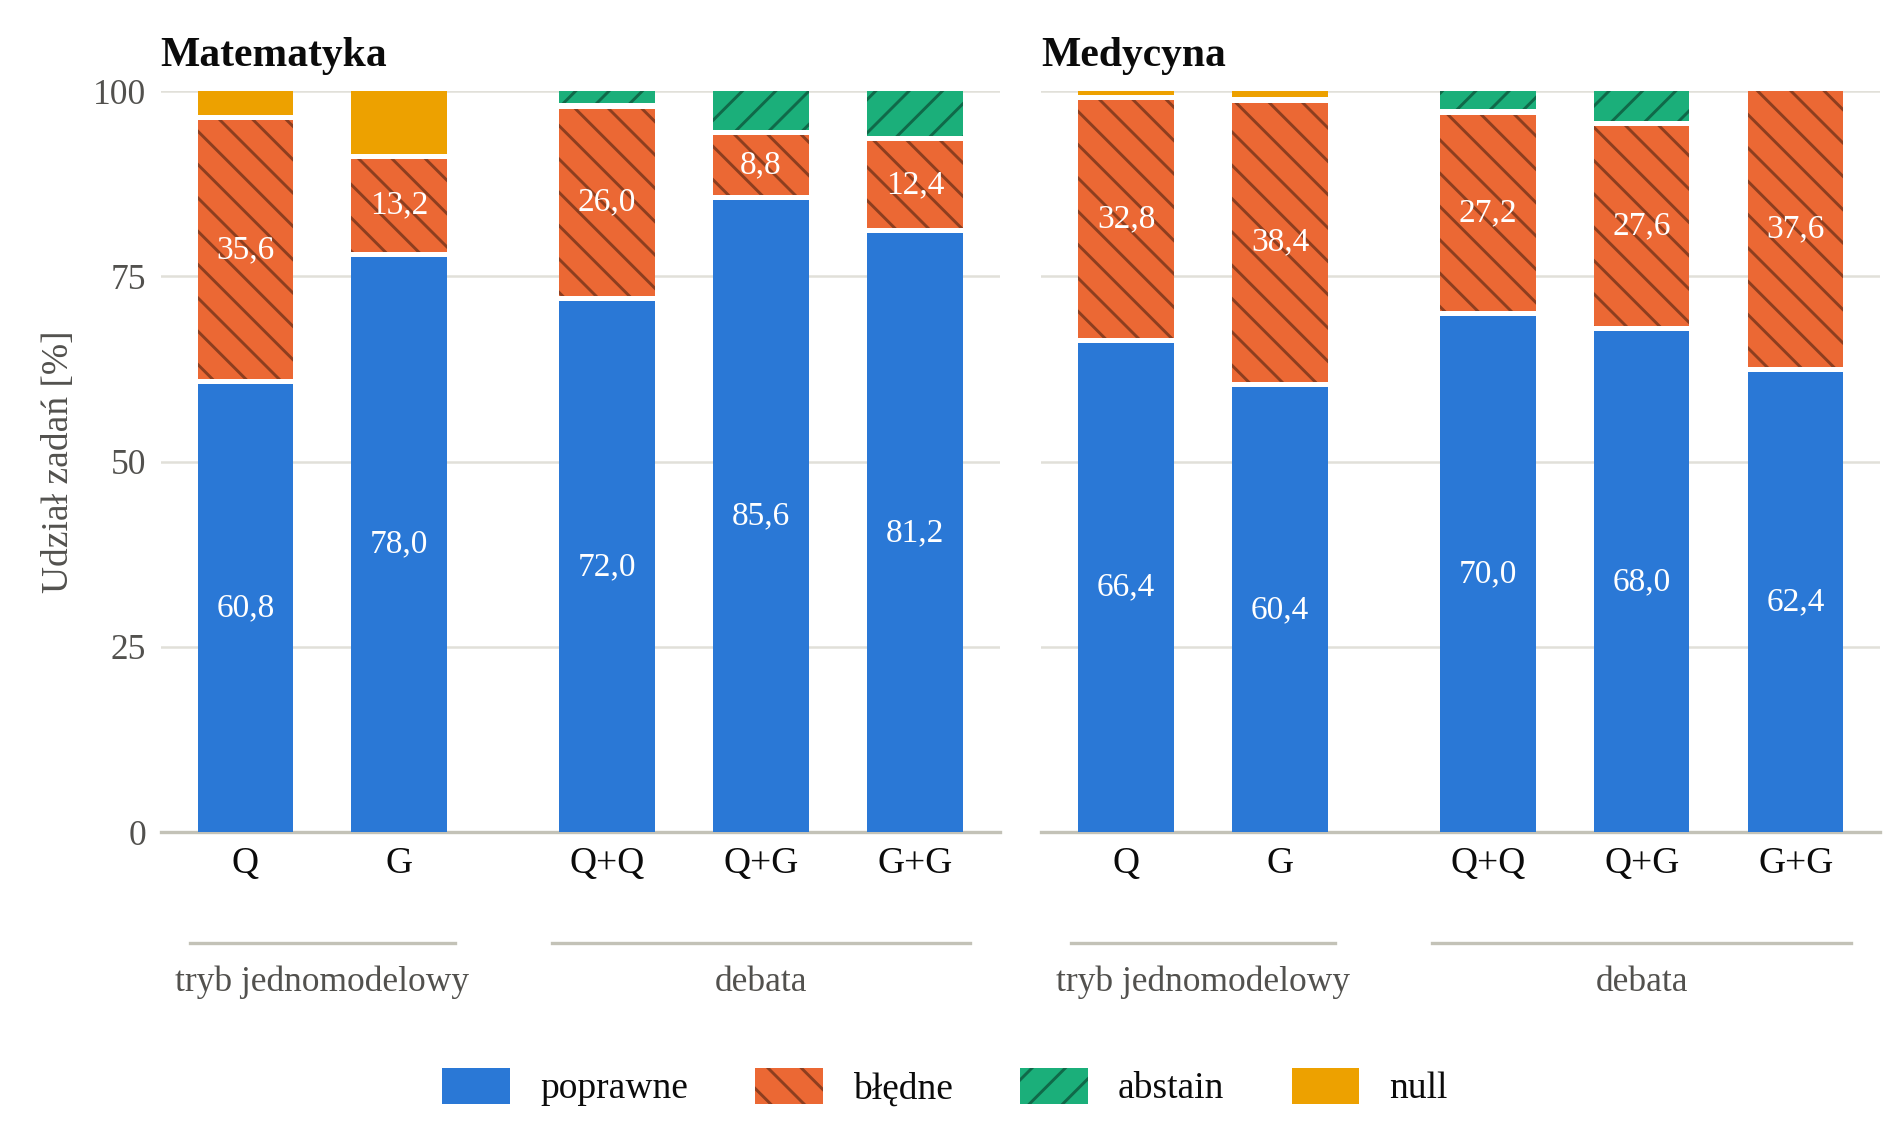
\includegraphics[width=\textwidth]{figures/rys-sklad-wynikow.png}
    \caption{Skład wyników w poszczególnych konfiguracjach: odsetek zadań poprawnych, błędnych, abstain i null ($n = 250$ zadań na zbiór)}
    \label{wyk:sklad_wynikow}
\end{wykres}

Rozpiętość wyników zależy od zbioru. W matematyce dokładność waha się od 60,8\% (Q) do 85,6\% (Q+G), czyli o 24,8 punktu procentowego (pp), a w medycynie od 60,4\% (G) do 70,0\% (Q+Q), czyli o 9,6~pp. Zbiór matematyczny pokazuje wyraźne różnice między konfiguracjami, natomiast w medycynie wszystkie leżą blisko siebie. Istotność tych różnic oceniono testem McNemara, a jej wyniki zestawia tabela~\ref{tab:testy_parowane}.

% !TEX root = ../main.tex
\begin{table}[H]
    \centering
    \caption[Porównania parami konfiguracji na tych samych zadaniach]{Porównania parami konfiguracji na tych samych zadaniach. A i B -- pierwsza i druga konfiguracja w kolumnie „Porównanie”; $\Delta$ -- różnica dokładności A $-$ B w punktach procentowych (pp); „tylko A” i „tylko B” -- zadania rozwiązane poprawnie wyłącznie przez daną konfigurację; $p$ -- dokładny test McNemara, pogrubiono $p < 0{,}05$. Lepszy solo: G w matematyce, Q w medycynie.}
    \label{tab:testy_parowane}
    \small
    \setlength{\tabcolsep}{2.5pt}
    \renewcommand{\arraystretch}{1.35}
    \sbox0{%
    \begin{tabular}{|>{\centering\arraybackslash}p{3.2cm}|>{\centering\arraybackslash}p{1.3cm}|>{\centering\arraybackslash}p{1.35cm}|>{\centering\arraybackslash}p{1.35cm}|>{\centering\arraybackslash}p{1.4cm}|>{\centering\arraybackslash}p{1.3cm}|>{\centering\arraybackslash}p{1.35cm}|>{\centering\arraybackslash}p{1.35cm}|>{\centering\arraybackslash}p{1.4cm}|}
        \hline
        \rowcolor{gray!20}
        \multicolumn{1}{|c|}{} & \multicolumn{4}{c|}{\textbf{Matematyka}} & \multicolumn{4}{c|}{\textbf{Medycyna}} \\ \cline{2-9}
        \rowcolor{gray!20}
        \textbf{Porównanie} & \textbf{$\Delta$ [pp]} & \textbf{tylko A} & \textbf{tylko B} & \textbf{p} & \textbf{$\Delta$ [pp]} & \textbf{tylko A} & \textbf{tylko B} & \textbf{p} \\ \hline
        Q+Q vs Q & $+$11,2 & 33 & 5 & \textbf{$<$0,001} & $+$3,6 & 13 & 4 & \textbf{0,049} \\ \hline
        G+G vs G & $+$3,2 & 11 & 3 & 0,057 & $+$2,0 & 10 & 5 & 0,302 \\ \hline
        Q+G vs lepszy solo & $+$7,6 & 22 & 3 & \textbf{$<$0,001} & $+$1,6 & 21 & 17 & 0,627 \\ \hline
        Q+G vs Q+Q & $+$13,6 & 43 & 9 & \textbf{$<$0,001} & $-$2,0 & 13 & 18 & 0,473 \\ \hline
        Q+G vs G+G & $+$4,4 & 17 & 6 & \textbf{0,035} & $+$5,6 & 29 & 15 & \textbf{0,049} \\ \hline
        G vs Q & $+$17,2 & 58 & 15 & \textbf{$<$0,001} & $-$6,0 & 25 & 40 & 0,082 \\ \hline
    \end{tabular}}
    \ifdim\wd0>\textwidth\sbox0{\resizebox{\textwidth}{!}{\usebox0}}\fi
    \usebox{0}
\end{table}


W matematyce G przewyższa Q o 17,2~pp ($p < 0{,}001$), chociaż 8,8\% zadań kończy się u niego wynikiem null (sekcja~\ref{sec:niepowodzenia}). Przewagę zawdzięcza małemu udziałowi odpowiedzi błędnych: 13,2\% wobec 35,6\% w Q. W medycynie kolejność jest odwrotna: Q jest lepszy o 6,0~pp (66,4\% wobec 60,4\%). Można przypuszczać, że modele mają mocne i słabe strony, na przykład G lepiej radzi sobie z rozumowaniem wieloetapowym, a Q z zadaniami wiedzowymi, jednak przeprowadzone eksperymenty tego jednoznacznie nie rozstrzygają.

Debata zmniejsza odsetek odpowiedzi błędnych. We wszystkich ośmiu porównaniach debaty z jej modelami składowymi (Q+Q z Q, G+G z G oraz Q+G z Q i z G, w obu zbiorach) udział błędnych był niższy, choć skala spadku była bardzo zróżnicowana. Q+Q zmniejsza go o 9,6~pp w matematyce i 5,6~pp w medycynie, Q+G względem modelu solo o mniejszym odsetku błędnych (G w matematyce, Q w medycynie) odpowiednio o 4,4 i 5,2~pp, a G+G zaledwie o 0,8~pp w obu zbiorach. O tym, czy spadek błędnych przekłada się na dokładność, decyduje zbiór. W matematyce Q+Q zyskuje 11,2~pp względem Q. W medycynie spadek odsetka błędnych w Q+G względem Q (5,2~pp) daje wzrost poprawnych tylko o 1,6~pp, a pozostałe 3,6~pp przechodzi w abstain (z 0,8\% null do 4,4\%). Przy przyjętej hierarchii wyników także jest to zyskiem: system rzadziej odpowiada błędnie, a częściej zgłasza brak zgody między modelami.

Debata mieszana Q+G jest najlepszą konfiguracją w matematyce: przewyższa G o 7,6~pp, Q+Q o 13,6~pp oraz G+G o 4,4~pp i ma najmniejszy odsetek błędnych (8,8\%). W medycynie jej wynik (68,0\%) jest wyższy niż Q (o 1,6~pp) i G+G (o 5,6~pp) oraz niższy niż Q+Q (o 2,0~pp). Żaden z testów nie wskazuje konfiguracji znacząco lepszej od Q+G. W obu zbiorach Q+G nie ustępuje więc najlepszemu modelowi solo, a w matematyce jest od niego istotnie lepsza. Nie wymaga przy tym wcześniejszego rozpoznania, który model pasuje do dziedziny, a zachowuje tę pozycję mimo udziału słabszego z dwóch modeli (Q w matematyce, G w medycynie). W tym sensie debata mieszana jest w obu badanych zbiorach rozwiązaniem najbardziej uniwersalnym, choć kosztem największego zużycia tokenów (sekcja~\ref{sec:koszt}).

\subsection{Kiedy debata pomaga}
\label{sec:kiedy_debata_pomaga}

Aby ustalić skąd w debacie biorą się zmiany wyniku, każde zadanie porównano z rundą niezależną, w której modele odpowiadają nie znając odpowiedzi drugiego. Tabela~\ref{tab:bilans_debaty} dzieli zadania na trzy rozłączne grupy: takie, w których modele zgodziły się od razu, a debata się nie odbyła, oraz dwie grupy zadań poddanych debacie: takie, w których w rundzie niezależnej żaden model nie podał poprawnej odpowiedzi, i takie, w których poprawną odpowiedź podał jeden z modeli. Gdy nie podał jej żaden, poprawny wynik końcowy oznacza zadanie uratowane, ponieważ debata musiała wytworzyć odpowiedź, której nikt wcześniej nie miał. Gdy podał ją jeden z modeli, debata powinna ją zachować, a wynik końcowy, który nie jest poprawny, oznacza zadanie utracone.

% !TEX root = ../main.tex
\begin{table}[H]
    \centering
    \caption[Bilans debaty względem rundy niezależnej]{Bilans debaty względem rundy niezależnej. Liczba zadań, dla każdej debaty $n = 250$. „Zgoda od razu” -- modele zgodziły się w rundzie niezależnej, więc debata się nie odbyła. „Uratowane” -- zadania z poprawnym wynikiem końcowym, gdy w rundzie niezależnej nikt nie miał poprawnej odpowiedzi; „utracone” -- zadania z niepoprawnym wynikiem końcowym (także abstain), gdy poprawną odpowiedź miał jeden z modeli.}
    \label{tab:bilans_debaty}
    \small
    \setlength{\tabcolsep}{2.5pt}
    \renewcommand{\arraystretch}{1.35}
    \sbox0{%
    \begin{tabular}{|>{\centering\arraybackslash}p{2.0cm}|>{\centering\arraybackslash}p{1.4cm}|>{\centering\arraybackslash}p{1.3cm}|>{\centering\arraybackslash}p{1.9cm}|>{\centering\arraybackslash}p{1.3cm}|>{\centering\arraybackslash}p{1.9cm}|>{\centering\arraybackslash}p{1.3cm}|>{\centering\arraybackslash}p{1.9cm}|}
        \hline
        \rowcolor{gray!20}
        \multicolumn{2}{|c|}{} & \multicolumn{2}{c|}{\shortstack{\textbf{Zgoda}\\\textbf{od razu}}} & \multicolumn{2}{c|}{\shortstack{\textbf{Żaden model}\\\textbf{poprawny}}} & \multicolumn{2}{c|}{\shortstack{\textbf{Jeden model}\\\textbf{poprawny}}} \\ \cline{3-8}
        \rowcolor{gray!20}
        \textbf{Zbiór} & \textbf{Debata} & \textbf{razem} & \textbf{w tym poprawna} & \textbf{razem} & \textbf{w tym uratowane} & \textbf{razem} & \textbf{w tym utracone} \\ \hline
        Matematyka & Q+Q & 185 & 134 & 37 & 19 & 28 & 1 \\ \cline{2-8}
         & Q+G & 141 & 132 & 36 & 10 & 73 & 1 \\ \cline{2-8}
         & G+G & 207 & 185 & 30 & 8 & 13 & 3 \\ \hline
        Medycyna & Q+Q & 220 & 163 & 7 & 0 & 23 & 11 \\ \cline{2-8}
         & Q+G & 160 & 129 & 16 & 1 & 74 & 34 \\ \cline{2-8}
         & G+G & 229 & 150 & 10 & 1 & 11 & 6 \\ \hline
    \end{tabular}}
    \usebox{0}
\end{table}


W matematyce debata działa w sposób naprawczy. We wszystkich trzech konfiguracjach debaty łącznie uratowano 37 ze 103 zadań, w których nikt nie miał poprawnej odpowiedzi w rundzie niezależnej. Spośród 114 zadań, w których poprawną odpowiedź w rundzie niezależnej miał jeden z modeli, poprawny wynik przetrwał w 96\% przypadków, a utracono 5. W medycynie jest odwrotnie: uratowano zaledwie 2 z 33 zadań, w których nikt nie miał poprawnej odpowiedzi w rundzie niezależnej. Z kolei spośród 108 zadań, w których ktoś ją miał, poprawny wynik przetrwał tylko w 53\% (57 zadań), a utracono 51 (w 13 utraconych debata skończyła się abstain). Utracone zadania mierzą skuteczność wyboru między odpowiedziami z rundy niezależnej, a nie stratę względem modelu solo, dlatego nie przeczą wynikowi z tabeli~\ref{tab:testy_parowane}, według którego debata w medycynie nie pogarsza dokładności. Można przypuszczać, że w matematyce poprawny tok rozumowania da się sprawdzić krok po kroku, więc argument modelu mającego rację ma szansę przekonać drugi, natomiast w MedMCQA odpowiedź zależy głównie od wiedzy, której debata nie uzupełni. Eksperymenty tego jednak nie rozstrzygają.

W większości zadań wynik ustala się jeszcze przed debatą: modele zgadzają się od razu w matematyce w 185 (Q+Q), 141 (Q+G) i 207 (G+G) zadaniach z 250, a w medycynie odpowiednio w 220, 160 i 229. Wiarygodność zgody zależy od składu pary. Dwa egzemplarze tego samego modelu częściej zgadzają się na odpowiedź błędną: w matematyce w 51 (Q+Q), 9 (Q+G) i 22 (G+G) zadaniach, a w medycynie odpowiednio w 57, 31 i 79. Wśród odpowiedzi uzgodnionych od razu, w debacie mieszanej poprawnych jest 94\% w matematyce i 81\% w medycynie, a w debatach jednorodnych 72\% (Q+Q) i 89\% (G+G) w matematyce oraz 74\% i 66\% w medycynie. Można przypuszczać, że błędy dwóch instancji jednego modelu są silniej skorelowane niż błędy dwóch różnych modeli.

Para mieszana częściej wchodzi w debatę: w matematyce w 109 zadaniach wobec 65 (Q+Q) i 43 (G+G), w medycynie w 90 wobec 30 i 21. O skutku decyduje zbiór. W matematyce poprawna odpowiedź przetrwała debatę prawie za każdym razem (Q+G: 72 z 73), a debata uratowała ponadto 10 zadań. Z tego względu większa liczba debat przekłada się tu na najlepszy wynik. W medycynie poprawna odpowiedź przetrwała debatę w obu parach w około połowie zadań (Q+Q: 12 z 23, Q+G: 40 z 74), w sytuacji gdy ktoś ją miał w rundzie niezależnej. Q+G utraciła więc więcej zadań (34 wobec 11 w Q+Q) głównie dlatego, że częściej debatowała. Te straty w przybliżeniu równoważą zysk z rzadszych zgodnych błędów (31 wobec 57 w Q+Q) i mogą tłumaczyć, dlaczego Q+G nie wyprzedza tam Q+Q. Większa liczba rund debaty jest też źródłem wyższego kosztu pary mieszanej (sekcja~\ref{sec:koszt}).

Abstain dotyczy zadań trudnych także dla pojedynczego modelu: odpowiedni model solo (Q dla Q+Q, G dla G+G, a dla Q+G lepszy z dwóch w danym zbiorze) rozwiązał poprawnie tylko 5 z 35 takich zadań w matematyce (14\%) i 5 z 18 w medycynie (28\%). Przyczyna jest jednak inna w obu zbiorach. W matematyce niemal każdy abstain towarzyszy uciętej generacji (sekcja~\ref{sec:niepowodzenia}), więc odzwierciedla głównie zadania wymagające długiego rozumowania, które nie mieszczą się w oknie 4096 tokenów, a nie świadome wstrzymanie się modeli. W medycynie ucięcie wystąpiło tylko w 1 z 18 przypadków, więc abstain oznacza tam rzeczywisty brak zgody między modelami i tylko tam można go traktować jako sygnał niepewności.

\subsection{Koszt}
\label{sec:koszt}

Koszt obliczeniowy rośnie wraz z liczbą modeli i rund. Koszt mierzono liczbą tokenów (prompt i generowana odpowiedź łącznie) oraz czasem rozwiązania zadania, uśrednionymi po wszystkich 250 zadaniach zbioru (tabela~\ref{tab:wyniki_zbiorcze}). W obu zbiorach debata zużywa od 2,4 do 4,7 razy więcej tokenów i od 1,9 do 4,5 razy więcej czasu niż odpowiadający jej model solo (dla debaty mieszanej przyjęto lepszy z dwóch modeli z tabeli~\ref{tab:wyniki_zbiorcze}). Konfiguracja mieszana zużywa najwięcej tokenów w obu zbiorach: 4,7 razy więcej niż G w matematyce i 4,2 razy więcej niż Q w medycynie, przy czasie dłuższym odpowiednio 3,7 i 4,5 razy. W matematyce najdłużej trwa jednak G+G (średnio 125,2~s na zadanie wobec 103,7~s dla Q+G). Zależność dokładności od kosztu przedstawiają wykresy~\ref{wyk:dokladnosc_koszt} (tokeny) i~\ref{wyk:dokladnosc_czas} (czas).

\begin{wykres}[H]
    \centering
    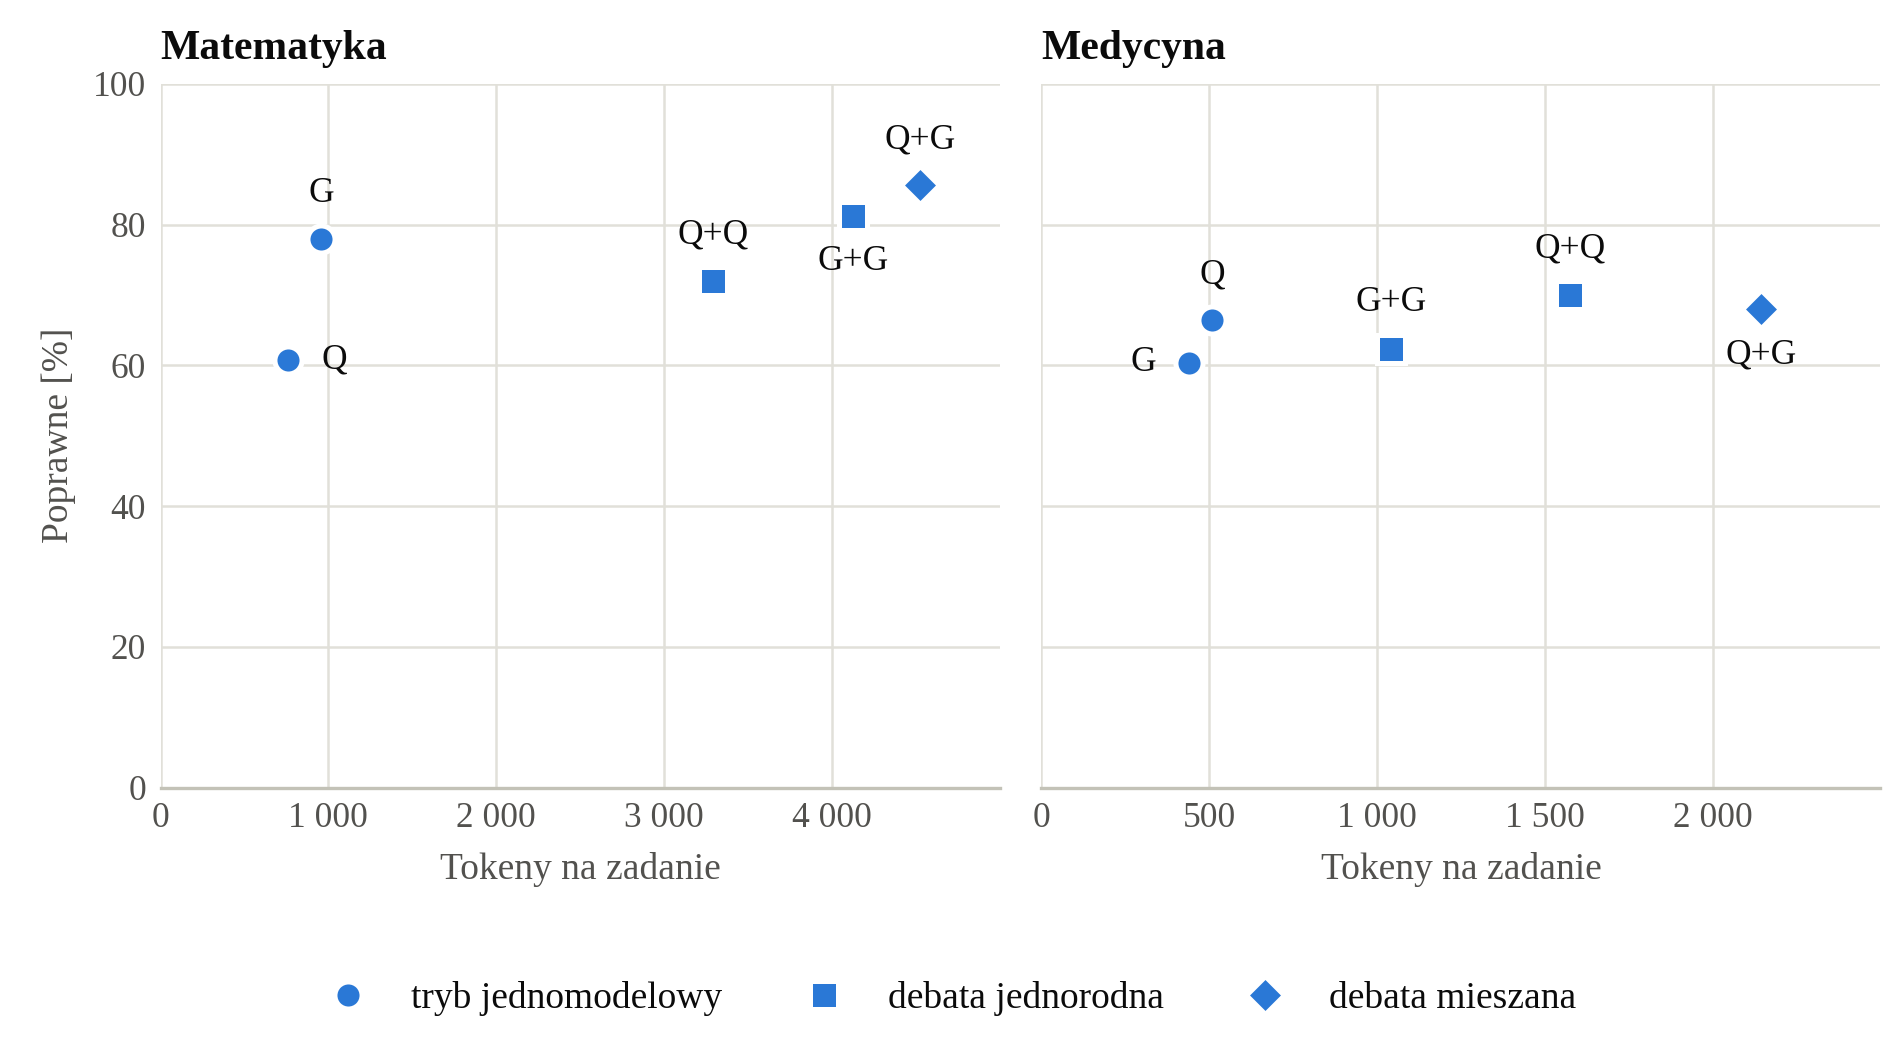
\includegraphics[width=\textwidth]{figures/rys-dokladnosc-koszt.png}
    \caption{Dokładność a liczba tokenów na zadanie w poszczególnych konfiguracjach}
    \label{wyk:dokladnosc_koszt}
\end{wykres}

\begin{wykres}[H]
    \centering
    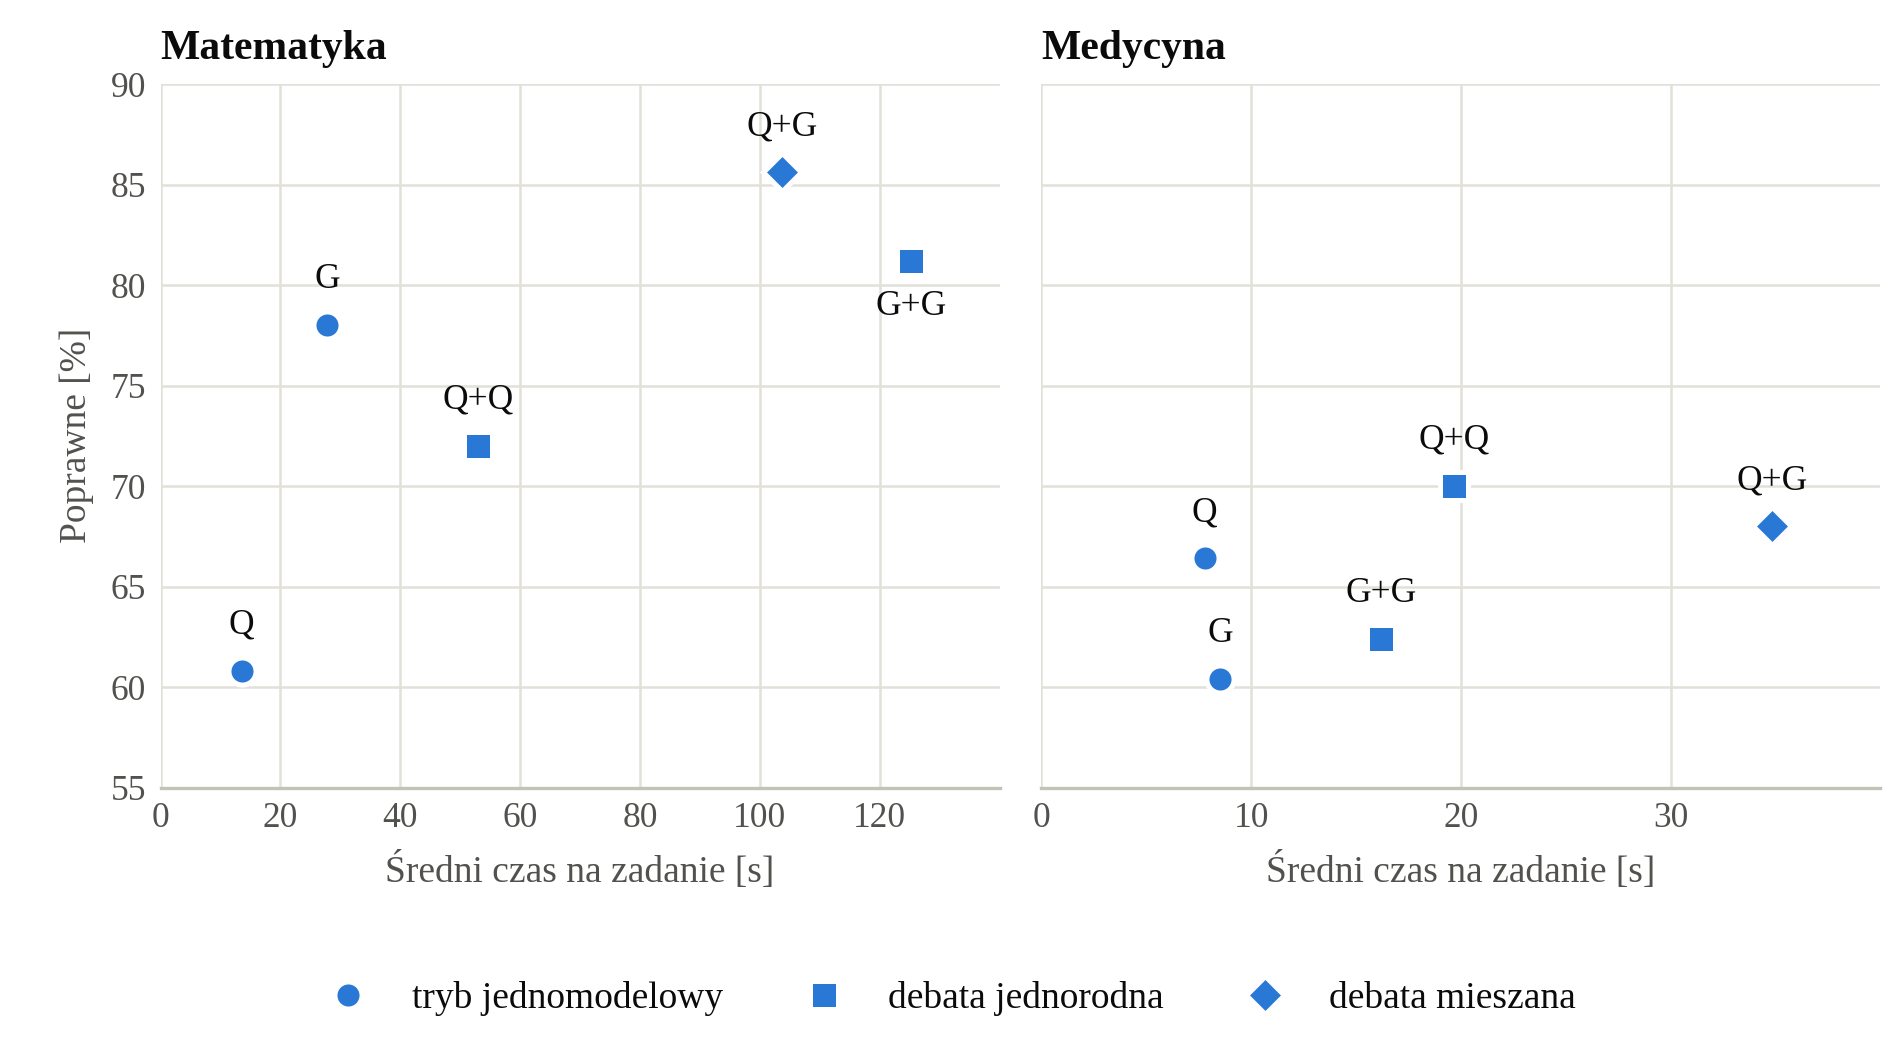
\includegraphics[width=\textwidth]{figures/rys-dokladnosc-czas.png}
    \caption{Dokładność a średni czas rozwiązania zadania w poszczególnych konfiguracjach}
    \label{wyk:dokladnosc_czas}
\end{wykres}

Czy ten koszt się zwraca, zależy od zbioru. W matematyce G jest dokładniejszy od Q+Q (78,0\% wobec 72,0\%), choć zużywa 3,4 razy mniej tokenów. Dopiero G+G i Q+G przewyższają go dokładnością, ale przy 4,3 i 4,7 razy większych kosztach. Istotny jest przy tym tylko zysk Q+G (7,6~pp, $p < 0{,}001$), a zysk G+G (3,2~pp, $p = 0{,}057$) tej istotności nie osiąga. W medycynie Q+Q poprawia wynik Q o 3,6~pp ($p = 0{,}049$) przy 3,1 razy większym koszcie, a Q+G zużywa 1,4 razy więcej tokenów niż Q+Q i nie ustępuje istotnie dokładnością (68,0\% wobec 70,0\%). Większy koszt debaty wyraźnie zwraca się więc tylko w matematyce.

Pod względem czasu w matematyce G nie ustępuje Q+Q dokładnością (78,0\% wobec 72,0\%), a rozwiązuje zadania 1,9 razy szybciej, natomiast Q+G jest dokładniejsza i szybsza od G+G (85,6\% w 103,7~s wobec 81,2\% w 125,2~s). G+G działa wolniej mimo mniejszej liczby tokenów (4100 wobec 4500), ponieważ model G przetwarza tokeny wolniej niż Q: w trybie solo zużywa 27,8~s przy 955 tokenach, a Q 13,5~s przy 760. W medycynie Q+G działa najwolniej (34,8~s) i 1,8 razy wolniej niż Q+Q, choć nie jest od niej dokładniejsza. Do tego czasu wlicza się średnio około 6--7~s na zadanie na ładowanie modeli przy przełączaniu między Q i G, którego praktycznie nie ma w pozostałych konfiguracjach.

Koszt debaty składa się z rundy niezależnej, w której oba modele odpowiadają jak w trybie solo, oraz z rund debaty. Runda niezależna zużywa 1600--2000~tokenów na zadanie w matematyce i 800--1000 w medycynie, czyli w przybliżeniu sumę kosztów obu modeli w trybie solo. Rundy debaty odpowiadają średnio za 55\% tokenów i 49\% czasu w matematyce oraz za 39\% tokenów i 30\% czasu w medycynie (średnie z trzech konfiguracji debaty).

W matematyce kolejne rundy nie są tańsze od pierwszej. W Q+G jedna runda kosztuje średnio 3800~tokenów i 65~s w rundzie 1 oraz 5200~tokenów i 118--126~s w rundach 2 i 3, ponieważ odpowiedzi modeli są w rundach 2 i 3 około dwa razy dłuższe niż w rundzie 1, a prompt, około czterokrotnie dłuższy niż w rundzie niezależnej, od rundy 1 już nie rośnie. W medycynie koszt rundy jest podobny w każdej z trzech (2100--2300~tokenów, 25--30~s). W Q+G odsetek poprawnych wyników wśród zadań, które kończą się w danej rundzie, spada w matematyce z 89\% w rundzie 1 do 70\% w rundzie 2 i 30\% w rundzie 3, a w medycynie z 60\% do 25\% i 18\%. Co najmniej połowa zadań, które doszły do rundy 3, kończy się abstain, a sama runda 3 zużywa 6--12\% wszystkich tokenów zadania (G+G w medycynie w ogóle do niej nie dochodzi). Można więc przypuszczać, że wydłużanie debaty ponad przyjęte trzy rundy byłoby mało opłacalne.

W obu zbiorach dokładniejszy jest model zużywający więcej tokenów: w matematyce G (955 tokenów na zadanie wobec 760 dla Q), w medycynie Q (508 wobec 440). W debacie mieszanej wzorzec się powtarza (matematyka: G 2400~tokenów wobec 2100 dla Q; medycyna: Q 1200 wobec 1000). Znaczną część kosztu stanowią wywołania ucięte po wyczerpaniu okna kontekstu (sekcja~\ref{sec:niepowodzenia}): w trybie solo 22 ucięte generacje G w matematyce zużywają 38\% tokenów, jakie G zużył na wszystkie 250 zadań tego zbioru, a w debatach w matematyce takie wywołania stanowią 24\% wszystkich tokenów w Q+Q, 37\% w Q+G i 57\% w G+G. W debatach w medycynie stanowią nie więcej niż 5,2\%.

\subsection{Niepowodzenia generacji i tryb rozumowania}
\label{sec:niepowodzenia}

Wynik null w trybie solo oznacza generację uciętą po wyczerpaniu okna kontekstu o długości 4096 tokenów, które obejmuje zarówno prompt, jak i generowany tekst. Takich wyników jest 36 na 1000 zadań rozwiązanych w trybie solo. Dotyczą głównie matematyki: rezultat null ma 3,6\% zadań Q i 8,8\% zadań G wobec 0,8\% i 1,2\% w medycynie, co zgadza się z tym, że zadania matematyczne wymagają dłuższych odpowiedzi: na jedno zadanie przypada tam średnio 760 (Q) i 955 (G) tokenów łącznie z promptem, wobec 508 i 440 w medycynie.

Debata nie zwraca wyniku null, ponieważ ucięta generacja oznacza w niej brak odpowiedzi jednego z modeli, a nie koniec zadania. Konsensus wymaga odpowiedzi od wszystkich modeli, więc debata przechodzi do kolejnej rundy, a po trzeciej kończy się abstain. W debatach matematycznych ucięcia są częstsze niż w trybie solo: dotyczą 6,9\% wywołań w Q+Q, 12,2\% w Q+G i 21,5\% w G+G wobec 3,6\% Q i 8,8\% G. Z kolei w medycynie stanowią 0,4--0,8\% wywołań. Zdarzają się też częściej w rundach debaty niż w rundzie niezależnej (w matematyce: w Q+Q 14,8\% wobec 3,8\%, w Q+G 20,9\% wobec 6,4\%, w G+G 55,3\% wobec 10,0\%). Prompt debaty zawiera odpowiedzi obu modeli z poprzedniej rundy (w uciętych wywołaniach średnio 1000--1600 tokenów wobec 300--400 w rundzie niezależnej), więc na generację zostaje mniej miejsca w tym samym oknie.

Ucięcia towarzyszą prawie każdemu abstain w matematyce. W 34 z 35 zadań zakończonych abstain co najmniej jedno wywołanie zostało ucięte. W 17 z tych 35 zadań wynik null zwrócił także odpowiedni model solo. W medycynie ucięcie wystąpiło tylko w 1 z 18 zadań zakończonych abstain. Abstain w tej dziedzinie wynika więc z braku zgody między modelami, a nie z braku odpowiedzi.

Sprawdzono też, czy włączenie trybu reasoning, w którym model przed odpowiedzią generuje osobną fazę rozumowania, poprawia wyniki. Tabela~\ref{tab:pilotaz_rozumowanie} zestawia wyniki dla niewielkiego podzbioru zadań z badania głównego: 10 pierwszych zadań w matematyce w każdej konfiguracji oraz 49 zadań z końca zbioru w medycynie (od 201. do 249., te same dla obu modeli).

% !TEX root = ../main.tex
\begin{table}[H]
    \centering
    \caption[Tryb bez rozumowania i z rozumowaniem na tych samych zadaniach]{Tryb bez rozumowania i z rozumowaniem na tych samych zadaniach. „Brak odpowiedzi” to null w trybie solo i abstain w debacie.}
    \label{tab:pilotaz_rozumowanie}
    \small
    \setlength{\tabcolsep}{2.5pt}
    \renewcommand{\arraystretch}{1.35}
    \sbox0{%
    \begin{tabular}{|>{\centering\arraybackslash}p{2.0cm}|>{\centering\arraybackslash}p{2.25cm}|>{\centering\arraybackslash}p{1.2cm}|>{\centering\arraybackslash}p{1.7cm}|>{\centering\arraybackslash}p{1.4cm}|>{\centering\arraybackslash}p{1.9cm}|>{\centering\arraybackslash}p{2.35cm}|>{\centering\arraybackslash}p{2.7cm}|}
        \hline
        \rowcolor{gray!20}
        \multicolumn{3}{|c|}{} & \multicolumn{5}{c|}{\textbf{bez rozumowania $\rightarrow$ z rozumowaniem}} \\ \cline{4-8}
        \rowcolor{gray!20}
        \textbf{Zbiór} & \textbf{Konfiguracja} & \textbf{Liczba zadań} & \textbf{Poprawne} & \textbf{Błędne} & \textbf{Brak odpowiedzi} & \textbf{Średni czas na zadanie [s]} & \textbf{Tokeny na zadanie} \\ \hline
        Matematyka & Q & 10 & 5 $\rightarrow$ 7 & 3 $\rightarrow$ 0 & 2 $\rightarrow$ 3 & 25,6 $\rightarrow$ 78,5 & 1\,191 $\rightarrow$ 2\,842 \\ \cline{2-8}
         & G & 10 & 8 $\rightarrow$ 4 & 1 $\rightarrow$ 0 & 1 $\rightarrow$ 6 & 25,5 $\rightarrow$ 130,7 & 898 $\rightarrow$ 3\,139 \\ \cline{2-8}
         & Q+Q & 10 & 6 $\rightarrow$ 8 & 4 $\rightarrow$ 0 & 0 $\rightarrow$ 2 & 54,9 $\rightarrow$ 384,5 & 2\,867 $\rightarrow$ 13\,233 \\ \cline{2-8}
         & Q+G & 10 & 9 $\rightarrow$ 5 & 1 $\rightarrow$ 0 & 0 $\rightarrow$ 5 & 121,8 $\rightarrow$ 649,9 & 4\,747 $\rightarrow$ 18\,208 \\ \cline{2-8}
         & G+G & 10 & 9 $\rightarrow$ 4 & 1 $\rightarrow$ 0 & 0 $\rightarrow$ 6 & 71,7 $\rightarrow$ 901,6 & 2\,398 $\rightarrow$ 21\,239 \\ \hline
        Medycyna & Q & 49 & 28 $\rightarrow$ 26 & 20 $\rightarrow$ 10 & 1 $\rightarrow$ 13 & 8,0 $\rightarrow$ 65,7 & 535 $\rightarrow$ 2\,585 \\ \cline{2-8}
         & G & 49 & 28 $\rightarrow$ 3 & 20 $\rightarrow$ 1 & 1 $\rightarrow$ 45 & 9,4 $\rightarrow$ 150,5 & 469 $\rightarrow$ 3\,843 \\ \hline
    \end{tabular}}
    \ifdim\wd0>\textwidth\sbox0{\resizebox{\textwidth}{!}{\usebox0}}\fi
    \usebox{0}
\end{table}


Rozumowanie prawie w całości eliminuje odpowiedzi błędne. W matematyce liczba błędnych odpowiedzi spada z 10 do 0 w pięciu konfiguracjach łącznie, a w medycynie z 20 do 10 w Q i z 20 do 1 w G. Nie oznacza to jednak poprawy wyników, bo jednocześnie rośnie liczba zadań bez odpowiedzi (w matematyce łącznie z 3 do 22). W trybie solo generacje często wyczerpywały okno kontekstowe: G w medycynie nie odpowiada w 45 z 49 zadań, a Q w 13 z 49. Poprawnych odpowiedzi przybywa tylko w Q i Q+Q w matematyce (o 2 zadania z 10), a w pozostałych konfiguracjach ich ubywa (w medycynie z 28 do 26 w Q i do 3 w G). Czas rozwiązywania zadań rośnie średnio ok. 8 razy, a liczba zużytych tokenów ok. 5 razy (np. G w medycynie zużywa 3843 tokenów na zadanie zamiast 469). Próba jest mała, więc różnice rzędu kilku zadań nie są pełnym dowodem. Wyniki z tabeli~\ref{tab:pilotaz_rozumowanie} pokazują, że przy oknie o długości 4096 tokenów faza rozumowania zajmuje tyle miejsca, że model często nie ma przestrzeni na podanie odpowiedzi. Wyniki nie pozwalają ocenić, czy rozumowanie pomogłoby przy większym oknie.

Poniższa analiza dotyczy wyłącznie próbki w trybie reasoning: tylko w niej generacja ma osobną fazę rozumowania, którą można przebadać, a ucięć w badaniu głównym (bez rozumowania) w ten sposób nie analizowano. W fazie rozumowania uciętych generacji G często powtarza się ten sam fragment tekstu słowo w słowo: w 74 ze 120 uciętych wywołań (w medycynie 38 z 45, w matematyce 36 z 75). W wywołaniach zakończonych powtórzenie takie wystąpiło w 2 z 21. Jeden z przykładów to generacja G na zadaniu z medycyny, w której w fazie rozumowania zdanie „Wait, I found a source! It's from a book on the behavior of birds.” powtarza się 120 razy. Słowa sygnalizujące poprawkę lub ponowne sprawdzenie (np. „Wait”, „Actually”) występują w uciętych generacjach w Q 1,2 razy częściej niż w zakończonych, a w uciętych generacjach G 5 razy częściej. Można przypuszczać, że w trybie reasoning G wyczerpuje okno przez zapętlenie, a Q przez samą długość rozumowania. Ocena opiera się na prostych miarach tekstu, a nie na wyczerpującej analizie.

% !TEX root = ../main.tex
\chapter{Podsumowanie}


%% -------------------- Bibliografia --------------------------
\clearpage
\phantomsection
\addcontentsline{toc}{chapter}{Wykaz literatury} % wpis do spisu treści
\label{page:Bibliography}
\printbibliography

%% -------------------- Wykaz wykresów ------------------------
%% (zastępuje wykaz rysunków — w pracy używane jest środowisko „wykres”)
\clearpage
\phantomsection
\addcontentsline{toc}{chapter}{Spis wykresów} % wpis do spisu treści
% !TEX root = ../main.tex
\listof{wykres}{Spis wykresów}

%% -------------------- Wykaz tabel ---------------------------
\renewcommand{\listtablename}{Wykaz tabel}
\clearpage
\phantomsection
\addcontentsline{toc}{chapter}{Wykaz tabel} % wpis do spisu treści
\listoftables

%% -------------------- Dodatki -------------------------------
%% przełączenie na tryb dodatków; każdy \include tworzy kolejny dodatek
\appendix
%% UWAGA: appendices/A_appendix.tex jest obecnie kopią appendices/_formatting.tex
%% (brak \chapter{...} z treścią) — jego dołączenie powoduje błąd ponownej
%% definicji \appchapter. Odkomentuj po wpisaniu treści dodatku.
% %% ============================================================
%% Formatowanie nagłówka: „Dodatek A: Tytuł” 
%% Automatyczne dodanie do spisu treści
%% Zawartość pozostaw bez zmian
%% ============================================================

% zachowujemy domyślne ustawienia \chapter do późniejszego użycia
\makeatletter
\let\OrigChapter\chapter

%% stworzenie nowego polecenia \appchapter z numeracją literową
\NewDocumentCommand{\appchapter}{ m o }{
  \refstepcounter{chapter}
  \setcounter{section}{0}
  \gdef\currentchaptertitle{#1}
  \OrigChapter*{Dodatek~\thechapter: #1} % dopisanie "Dodatek" do tytułu
  \chaptermark{#1}
  \phantomsection
  \addcontentsline{toc}{chapter}{Dodatek~\thechapter: #1} % dodanie do spisu treści
  \IfNoValueF{#2}{\label{#2}}
}

%% po poleceniu \appendix
%% \chapter{...} korzysta z \appchapter,
%% \chapter*{...} działa jak dotąd (bez numeru w spisie treści).
\pretocmd{\appendix}{
  \let\OrigChapter\chapter
  \renewcommand{\chapter}{
    \@ifstar{\OrigChapter*}{\appchapter}
  }
}{}{}
\makeatother


\end{document}
